
\documentclass[12pt,a4paper]{report}
\usepackage[T1]{fontenc}
\usepackage{lmodern}
\usepackage[protrusion=true,expansion=false]{microtype}

% Centralized geometry setup
\usepackage[a4paper, top=2.0cm, bottom=2.2cm, left=1.8cm, right=1.8cm, headheight=16pt, headsep=12pt, footskip=22pt, includeheadfoot]{geometry}

\usepackage{graphicx}
\usepackage{amsmath}
\usepackage{amssymb}
\usepackage{booktabs}
\usepackage{array}
\usepackage{tabularx}
\usepackage{float}
\usepackage{fancyhdr}
\usepackage{xcolor}
\usepackage{setspace}
\usepackage{enumitem}
\usepackage{caption}

\captionsetup{
    labelfont=bf,
    justification=raggedright,
    singlelinecheck=false,
    format=plain
}
\usepackage{subcaption}
\usepackage{multirow}
\usepackage{colortbl}
\usepackage{hhline}
\usepackage{longtable}
\setlength{\LTleft}{\fill}
\setlength{\LTright}{\fill}
\usepackage{titlesec}
\usepackage{titletoc}
\usepackage{lastpage}
\usepackage{makecell}
\usepackage{etoolbox}
\usepackage{needspace}

% Preamble color definitions and table metrics from single source of truth
% OsdagBridge centralized palette definitions
\definecolor{OsdagPrimary}{HTML}{16331C}
\definecolor{OsdagAccent}{HTML}{5E8014}
\definecolor{OsdagGreen}{HTML}{789A1B}
\definecolor{OsdagGreenLight}{HTML}{EBF2DE}
\definecolor{OsdagHeaderBg}{HTML}{EBF2DE}
\definecolor{OsdagZebra}{HTML}{F7FAF3}
\definecolor{OsdagPass}{HTML}{226B28}
\definecolor{OsdagFail}{HTML}{B91C1C}
\definecolor{OsdagBorder}{HTML}{CCD7C5}
\definecolor{OsdagMuted}{HTML}{455443}
% Legacy alias to maintain backward compatibility
\definecolor{osdagGreen}{HTML}{789A1B}

% Centralized table geometry and padding
\setlength{\tabcolsep}{4.5pt}
\renewcommand{\arraystretch}{1.15}
\setlength{\LTpre}{4pt}
\setlength{\LTpost}{5pt}
\setlength{\arrayrulewidth}{0.45pt}
\setlength{\extrarowheight}{1.0pt}
\arrayrulecolor{OsdagBorder}


\numberwithin{table}{chapter}
\numberwithin{figure}{chapter}

% Prevent tables from overflowing past the page bottom or leaving ghost headers:
% if fewer than 10 baseline-skips remain, break to the next page first.
\BeforeBeginEnvironment{table}{\Needspace{6\baselineskip}}
\BeforeBeginEnvironment{longtable}{\Needspace{10\baselineskip}}

\fancypagestyle{main}{
  \fancyhf{}
  \fancyhead[L]{\footnotesize\textcolor{OsdagMuted}{\textbf{\color{OsdagPrimary}OsdagBridge} \quad\textbar\quad \textit{Short Span Steel Girder Bridge}}}
  \fancyhead[R]{\footnotesize\textcolor{OsdagMuted}{Job: \textbf{\color{OsdagPrimary}{JOB-2026-001}} \quad\textbar\quad 2026-11-22}}
  \fancyfoot[L]{\footnotesize\color{OsdagMuted}Osdag \quad\textbar\quad FOSSEE \quad\textbar\quad Indian Institute of Technology Bombay}
  \fancyfoot[R]{\footnotesize\color{OsdagMuted}Page \textbf{\thepage} of \pageref{LastPage}}
  \renewcommand{\headrule}{{\color{OsdagGreen}\hrule width\headwidth height 1.0pt}\vspace{2pt}}
  \renewcommand{\footrule}{%
    \ifbool{hasSDonPage}{%
      \vspace{-16pt}%
      \hbox to \headwidth{\textcolor{OsdagMuted}{\footnotesize\textit{* Software default value}}\hfil}%
      \vspace{4pt}%
    }{%
      \vspace{-4pt}%
    }%
    \color{OsdagBorder}\hrule width\headwidth height 0.5pt \vspace{4pt}%
  }
}
\fancypagestyle{plain}{
  \fancyhf{}
  \fancyhead[L]{\footnotesize\textcolor{OsdagMuted}{\textbf{\color{OsdagPrimary}OsdagBridge} \quad\textbar\quad \textit{Short Span Steel Girder Bridge}}}
  \fancyhead[R]{\footnotesize\textcolor{OsdagMuted}{Job: \textbf{\color{OsdagPrimary}{JOB-2026-001}} \quad\textbar\quad 2026-11-22}}
  \fancyfoot[L]{\footnotesize\color{OsdagMuted}Osdag \quad\textbar\quad FOSSEE \quad\textbar\quad Indian Institute of Technology Bombay}
  \fancyfoot[R]{\footnotesize\color{OsdagMuted}Page \textbf{\thepage} of \pageref{LastPage}}
  \renewcommand{\headrule}{{\color{OsdagGreen}\hrule width\headwidth height 1.0pt}\vspace{2pt}}
  \renewcommand{\footrule}{%
    \ifbool{hasSDonPage}{%
      \vspace{-16pt}%
      \hbox to \headwidth{\textcolor{OsdagMuted}{\footnotesize\textit{* Software default value}}\hfil}%
      \vspace{4pt}%
    }{%
      \vspace{-4pt}%
    }%
    \color{OsdagBorder}\hrule width\headwidth height 0.5pt \vspace{4pt}%
  }
}
\fancypagestyle{firstpage}{
  \fancyhf{}
  \renewcommand{\headrulewidth}{0pt}
  \renewcommand{\footrulewidth}{0pt}
}
\pagestyle{main}
\setstretch{1.04}

% Column Types
\newcolumntype{L}[1]{>{\raggedright\arraybackslash}p{#1}}
\newcolumntype{C}[1]{>{\centering\arraybackslash}p{#1}}
\newcolumntype{R}[1]{>{\raggedleft\arraybackslash}p{#1}}

% Hyperref loaded strictly last with bookmark and navigation metadata
\usepackage[
  bookmarks=true,
  bookmarksnumbered=true,
  bookmarksopen=true,
  colorlinks=true,
  linkcolor=OsdagPrimary,
  citecolor=OsdagAccent,
  urlcolor=OsdagAccent,
  pdftitle={Short Span Steel Girder Bridge - OsdagBridge Design Report},
  pdfauthor={OsdagBridge (IIT Bombay / FOSSEE) | Contributor: John Varghese (J0X)},
  pdfsubject={Bridge Superstructure Structural Design and Verification Report},
  pdfkeywords={Osdag, OsdagBridge, Bridge Design, Plate Girder, IRC 22:2015, IRC 6:2017, IS 800:2007, FOSSEE, IIT Bombay, Contributor: John Varghese},
  pdfcreator={OsdagBridge LaTeX Report Generator}
]{hyperref}

% Software-default asterisk
\newcommand{\sdstar}{\textsuperscript{*}}
\newbool{hasSDonPage}
\boolfalse{hasSDonPage}
\newcommand{\markSD}{\global\booltrue{hasSDonPage}}
\renewcommand{\sdstar}{\textsuperscript{*}\markSD{}}
\AddToHook{shipout/before}{\global\boolfalse{hasSDonPage}}

\title{\Large\textbf{OsdagBridge} \\ \normalsize Open Source Software for Steel Girder Bridge Design \\ \vspace{2cm} \large Design Report}
\author{}
\date{}

\begin{document}


\begin{titlepage}
\thispagestyle{empty}
\noindent
\begin{minipage}[b]{0.64\linewidth}
{\scriptsize\bfseries\color{OsdagAccent}\textsc{Structural Engineering Design \& Verification Report}}
\end{minipage}%
\begin{minipage}[b]{0.36\linewidth}
\raggedleft
{\scriptsize\color{OsdagMuted}\textbf{JOB:} JOB-2026-001 \quad\textbar\quad 2026-11-22}
\end{minipage}\\[3pt]
{\color{OsdagGreen}\rule{\linewidth}{2.0pt}}\\[0.4cm]

\noindent
\begin{center}

\includegraphics[height=1.9cm,keepaspectratio]{assets/osdag_logo.png}
\end{center}
\vspace{0.2cm}

\begin{center}
{\fontsize{21}{25}\selectfont \textbf{\color{OsdagPrimary}Short Span Steel Girder Bridge}}\\[0.2cm]
{\normalsize\color{OsdagMuted}Open Source Software for Steel Girder Bridge Design}\\[0.15cm]
{\small\bfseries\color{OsdagGreen}Detailed Structural Design \& Verification Report}\\[0.4cm]
\end{center}

\noindent
\begin{center}
\renewcommand{\arraystretch}{1.20}
\setlength{\tabcolsep}{6pt}
\begin{tabular}{|>{\bfseries\color{OsdagPrimary}\raggedright\arraybackslash}m{4.2cm}|>{\raggedright\arraybackslash}m{9.8cm}|}
\hline
\rowcolor{OsdagHeaderBg}
\multicolumn{2}{|l|}{\textbf{\color{OsdagPrimary}PROJECT METADATA \& RECORD}} \\
\hline
Project Name & Short Span Steel Girder Bridge \\
\hline
\rowcolor{OsdagZebra}
Project Location & Indore, Madhya Pradesh \\
\hline
Author / Designer & Structural Design Engineer \\
\hline
\rowcolor{OsdagZebra}
Reviewer & Chief Structural Engineer \\
\hline
Organization & Osdag \\
\hline
\rowcolor{OsdagZebra}
Client & IIT Bombay \\
\hline
Job Number & JOB-2026-001 \\
\hline
\rowcolor{OsdagZebra}
Date of Issue & 2026-11-22 \\
\hline
Report Version & Rev 1.0 \\
\hline
\end{tabular}
\end{center}

\vfill
\noindent
\begin{center}
{\footnotesize\color{OsdagMuted}Developed by \textbf{\color{OsdagPrimary}Osdag Project} \ \textbar\ \ Supported by \textbf{FOSSEE} \ \textbar\ \ \textbf{Indian Institute of Technology Bombay}}
\end{center}
\vspace*{0.2cm}
\end{titlepage}
\setcounter{page}{2}


% Chapter / TOC Formatting
\titleformat{\chapter}[hang]
  {\normalfont\LARGE\bfseries\color{OsdagPrimary}}
  {\color{OsdagGreen}\thechapter\quad\textcolor{OsdagBorder}{|}\quad}{0pt}{}
\titlespacing*{\chapter}{0pt}{16pt}{10pt}

\titleformat{name=\chapter,numberless}[hang]
  {\normalfont\LARGE\bfseries\color{OsdagPrimary}}{}{0pt}{}

\titleformat{\section}[hang]
  {\normalfont\Large\bfseries\color{OsdagPrimary}}
  {\color{OsdagAccent}\thesection\quad}{0pt}{}
\titlespacing*{\section}{0pt}{10pt}{5pt}

\titleformat{\subsection}[hang]
  {\normalfont\large\bfseries\color{OsdagAccent}}
  {\thesubsection\quad}{0pt}{}
\titlespacing*{\subsection}{0pt}{6pt}{3pt}

\setcounter{tocdepth}{2}

% TOC styling using titletoc
\titlecontents{chapter}[1.8em]
  {\normalfont\bfseries\vspace{2pt}\color{OsdagPrimary}}
  {\contentslabel{1.8em}}
  {\hspace*{-1.8em}}
  {\hfill\contentspage}

\titlecontents{section}[4.2em]
  {\normalfont\color{OsdagMuted}}
  {\contentslabel{2.4em}}
  {\hspace*{-2.4em}}
  {\hfill\contentspage}

\titlecontents{subsection}[7.2em]
  {\normalfont\footnotesize\color{OsdagMuted}}
  {\contentslabel{3.0em}}
  {\hspace*{-3.0em}}
  {\hfill\contentspage}

\newpage
\renewcommand{\contentsname}{\centering\LARGE\bfseries\color{OsdagPrimary} Table of Contents}
\tableofcontents


\newpage
{\centering\Large\bfseries\color{OsdagPrimary} Executive Summary\par}
\addcontentsline{toc}{chapter}{Executive Summary}
\vspace{0.8em}

% Executive Summary Callout Box
\begin{center}
\setlength{\fboxsep}{12pt}
\setlength{\fboxrule}{0.8pt}
\fcolorbox{OsdagBorder}{OsdagZebra}{%
\parbox{0.95\linewidth}{%
{\color{OsdagGreen}\rule{\linewidth}{2.0pt}}\\[8pt]
\centering
{\large\bfseries\color{OsdagPrimary} EXECUTIVE DESIGN SUMMARY}\\[8pt]
\begin{tabular}{@{}p{0.48\linewidth}p{0.50\linewidth}@{}}
\textbf{Structure:} Plate Girder Highway Bridge & \textbf{Overall Status:} \textbf{\color{OsdagFail}{UNSAFE (FAIL)}} \\[5pt]
\textbf{Span:} 24 m \quad\textbar\quad \textbf{Carriageway:} 7.5 m & \textbf{Controlling UR:} \textbf{1.97 (Girder)} \\[5pt]
\textbf{Girders:} 4 \quad\textbar\quad \textbf{Spacing:} 2.1 m & \textbf{Governing Check:} Fatigue Normal Stress \\[5pt]
\textbf{Design Codes:} IRC 5, 6, 22, 24, IS 800 & \textbf{Deck Thickness:} 250.0 mm \\[2pt]
\end{tabular}
}}
\end{center}

\vspace{0.8em}
This section provides a concise summary of the bridge design, key inputs, governing loads, and final design outcomes.

\section*{Project Overview}
\addcontentsline{toc}{section}{Project Overview}
\label{sec:project-overview}

\begin{tabular}{|L{5.5cm}|L{8.5cm}|}
\hline
\rowcolor{OsdagHeaderBg}
\textbf{Parameter} & \textbf{Design Specification} \\
\hline
\textbf{Bridge Type} & Highway Bridge \\
\hline
\textbf{Design Standards} & IRC 5:2015, IRC 6:2017, IRC 22:2015, IRC 24:2010, IS 800:2007 \\
\hline
\textbf{Span (m)} & 24 \\
\hline
\textbf{Carriageway Width (m)} & 7.5 \\
\hline
\textbf{No. of Girders} & 4 \\
\hline
\textbf{Girder Spacing (m)} & 2.1 \\
\hline
\textbf{Deck Thickness (mm)} & 250.0 \\
\hline
\textbf{Overall Design Status} & UNSAFE (FAIL: Fatigue Normal Stress, Intermediate Stiffener Outstand Limit, Fatigue Shear Stress) \\
\hline
\textbf{Governing Check} & Fatigue Normal Stress \\
\hline
\textbf{Overall Utilization Ratio (max)} & 1.97 \\
\hline
\end{tabular}

\vspace{1em}
\begin{figure}[H]
\centering
\includegraphics[width=0.9\textwidth]{/tmp/tmpo186htwv/images/girder_top.png}
\caption{\small Overall Bridge Plan}
\end{figure}

\newpage

\begin{figure}[H]
\centering
\includegraphics[width=0.9\textwidth]{/tmp/tmpo186htwv/images/cross_section.png}
\caption{\small Typical Cross-Section (with girder, deck, barriers, footpath)}
\end{figure}

\begin{figure}[H]
\centering
\includegraphics[width=0.9\textwidth]{/tmp/tmpo186htwv/images/final_geometry.png}
\caption{\small 3D View of Bridge Superstructure}
\end{figure}

\clearpage
\Needspace{8\baselineskip}
\begin{longtable}{|C{1.8cm}|C{2.0cm}|C{4.4cm}|L{6.2cm}|C{2.0cm}|}
\caption{\textbf{Final Bridge Geometry (after optimization)}}\label{tab:final-bridge-geometry} \\
\hline
\rowcolor{OsdagHeaderBg}
\textbf{Girder} & \textbf{Member ID} & \textbf{Section Designation} & \textbf{Governing Check} & \textbf{Utilization Ratio} \\[6pt]
\hline
\endfirsthead
\multicolumn{5}{c}{\small\textit{Final Bridge Geometry (after optimization) (continued from previous page)}} \\[4pt]
\hline
\rowcolor{OsdagHeaderBg}
\textbf{Girder} & \textbf{Member ID} & \textbf{Section Designation} & \textbf{Governing Check} & \textbf{Utilization Ratio} \\[6pt]
\hline
\endhead
\hline
\multicolumn{5}{r}{\small\textit{Continued on next page}} \\
\endfoot
\hline
\endlastfoot
G1 & G1M1 & 1340 $\times$ 410 $\times$ 18 $\times$ 410 $\times$ 18 & Fatigue Normal Stress & 1.95 \\[6pt]
\hline
G2 & G2M1 & 1340 $\times$ 410 $\times$ 18 $\times$ 410 $\times$ 18 & Fatigue Normal Stress & 1.96 \\[6pt]
\hline
G3 & G3M1 & 1340 $\times$ 410 $\times$ 18 $\times$ 410 $\times$ 18 & Fatigue Normal Stress & 1.97 \\[6pt]
\hline
G4 & G4M1 & 1340 $\times$ 410 $\times$ 18 $\times$ 410 $\times$ 18 & Fatigue Normal Stress & 1.97 \\[6pt]
\hline
\end{longtable}


\vspace{0.4em}
\noindent\textit{Note: Utilization ratio (UR) = demand / capacity. A value $\le 1.0$ indicates a passing check.}

\vspace{1em}

\section*{Key Design Outcomes Summary}
\addcontentsline{toc}{section}{Key Design Outcomes Summary}
\label{sec:key-outcomes}

\begin{itemize}[leftmargin=1.5em, itemsep=4pt]
\item \textbf{Steel Plate Girders:} \textbf{\color{OsdagFail}{FAIL}} (Fatigue Normal Stress, Int.Stiff:\allowbreak{} Leg $\le$ H\_\allowbreak{}limit, Fatigue Shear Stress)
\item \textbf{Concrete Deck Slab:} \textbf{\color{OsdagPass}{PASS}}
\item \textbf{Cross Bracing System:} \textbf{\color{OsdagPass}{PASS}}
\item \textbf{End Diaphragms:} \textbf{\color{OsdagMuted}{N/A}}
\end{itemize}

\section*{Design Assumptions and Limitations}
\addcontentsline{toc}{section}{Design Assumptions and Limitations}
\label{sec:assumptions}

\begin{itemize}
\item Additional inputs not provided by the user were assumed by software per IRC/IS code defaults or practical consideration.
\item Grillage analysis was performed using OSPGrillage assuming simply supported I-girders.
\item Substructure and foundation design are not included in this report.
\item Splice connections and bearings are not designed in this version.
\end{itemize}

% Restore numbered chapter format
\titleformat{\chapter}[block]{\normalfont\Large\bfseries\centering}{\thechapter}{1em}{}
\titlespacing*{\chapter}{0pt}{-30pt}{10pt}


\chapter{Project Information}

This section records all project metadata as entered by the designer.

\section{Project and Design Team Details}
\label{sec:project-details}

\begin{tabular}{|L{5.5cm}|L{8.5cm}|}
\hline
\rowcolor{OsdagHeaderBg}
\textbf{Parameter} & \textbf{Design Specification} \\
\hline
\textnormal{Project Name} & Short Span Steel Girder Bridge \\
\hline
\rowcolor{OsdagZebra}
\textnormal{Project Location} & Indore, Madhya Pradesh \\
\hline
\textnormal{Designer} & Structural Design Engineer \\
\hline
\rowcolor{OsdagZebra}
\textnormal{Reviewer} & Chief Structural Engineer \\
\hline
\textnormal{Organization} & Osdag \\
\hline
\rowcolor{OsdagZebra}
\textnormal{Client} & IIT Bombay \\
\hline
\textnormal{Software Version} & OsdagBridge \\
\hline
\end{tabular}


\section{Applicable Codes and Standards}
\label{sec:codes}

\begin{itemize}[leftmargin=1.5em, itemsep=2pt]
\item \textbf{IRC 5:2015} - Standard Specifications and Code of Practice for Road Bridges, Section I: General Features of Design
\item \textbf{IRC 6:2017} - Standard Specifications and Code of Practice for Road Bridges, Section II: Loads and Load Combinations
\item \textbf{IRC 22:2015} - Standard Specifications and Code of Practice for Road Bridges, Section VI: Composite Construction (Limit State Method)
\item \textbf{IRC 24:2010} - Standard Specifications and Code of Practice for Road Bridges, Section V: Steel Road Bridges (Limit State Method)
\item \textbf{IRC 112:2020} - Code of Practice for Concrete Road Bridges (Deck Slab Design)
\item \textbf{IRC SP 114:2018} - Guidelines for Seismic Design of Road Bridges
\item \textbf{IS 800:2007} - General Construction in Steel - Code of Practice
\item \textbf{IS 2062:2011} - Hot Rolled Medium and High Tensile Structural Steel - Specification
\end{itemize}

\vspace{0.8em}
\section{Nomenclature and Acronyms}
\label{sec:nomenclature}

\begingroup
\small
\begin{longtable}{|C{2.6cm}|L{11.4cm}|}
\hline
\rowcolor{OsdagHeaderBg}
\textbf{Term / Acronym} & \textbf{Engineering Definition} \\[6pt]
\hline
\endfirsthead
\multicolumn{2}{c}{\small\textit{Nomenclature and Acronyms (continued from previous page)}} \\[4pt]
\hline
\rowcolor{OsdagHeaderBg}
\textbf{Term / Acronym} & \textbf{Engineering Definition} \\[6pt]
\hline
\endhead
\hline
\multicolumn{2}{r}{\small\textit{Continued on next page}} \\
\endfoot
\hline
\endlastfoot
SW & Self-Weight (Dead load of structural members) \\[4pt]
\hline
\rowcolor{OsdagZebra}
DW & Dead Load of Surfacing and Superimposed Dead Load (Wearing Course) \\[4pt]
\hline
SIDL & Superimposed Dead Load (Crash barriers, railings, utilities) \\[4pt]
\hline
\rowcolor{OsdagZebra}
LL & Vehicular Live Load (IRC Class A, 70R, Special Vehicles) \\[4pt]
\hline
WL & Wind Load evaluated per IRC 6:2017 Clause 209 \\[4pt]
\hline
\rowcolor{OsdagZebra}
EL / EQ & Earthquake / Seismic Load evaluated per IRC 6 and IRC SP 114 \\[4pt]
\hline
TL & Temperature Load (Thermal range, rise, and fall) per IRC 6 \\[4pt]
\hline
\rowcolor{OsdagZebra}
ITS & Intermediate Transverse Stiffeners \\[4pt]
\hline
LTB & Lateral Torsional Buckling of steel flexural members \\[4pt]
\hline
\rowcolor{OsdagZebra}
ULS & Ultimate Limit State (Strength, stability, and equilibrium) \\[4pt]
\hline
SLS & Serviceability Limit State (Deflection, crack width, stress limits, fatigue) \\[4pt]
\hline
\rowcolor{OsdagZebra}
UR / DCR & Utilization Ratio / Demand-to-Capacity Ratio (Demand / Capacity $\le$ 1.0) \\[4pt]
\hline
BoQ & Bill of Quantities / Material Take-off \\[4pt]
\hline
\rowcolor{OsdagZebra}
c/c & Centre-to-Centre dimension spacing \\[4pt]
\hline
\end{longtable}
\endgroup


\chapter{Input Parameters}

\setlength{\abovecaptionskip}{2pt}
\setlength{\belowcaptionskip}{2pt}

This section documents all inputs provided to OsdagBridge. User-provided inputs are clearly distinguished from software-assumed defaults. Where the user did not supply a value, the software has applied the IRC/IS code default or an empirical guideline; these are annotated with an asterisk (\sdstar{}).

\section{Basic Inputs (User-Defined)}
\label{sec:basic-inputs}

\noindent\textit{Note: These inputs are mandatory and were provided by the user.}

\begin{table}[H]
\caption{\textbf{Project Location}}
\label{subsec:project-location}
\begin{tabular}{|L{5.5cm}|L{8.5cm}|}
\hline
\rowcolor{OsdagHeaderBg}
\textbf{Parameter} & \textbf{Value} \\
\hline
\textnormal{Project Location} & Indore, Madhya Pradesh \\
\hline
\rowcolor{OsdagZebra}
\textnormal{Latitude / Longitude} & 22.7196, 75.8577 \\
\hline
\textnormal{Seismic Zone (IRC 6)} & II \\
\hline
\rowcolor{OsdagZebra}
\textnormal{Basic Wind Speed (IRC 6)} & 39 m/s \\
\hline
\textnormal{Shade Temp. Max / Min (IRC 6)} & 46 °C / -2.8 °C \\
\hline
\end{tabular}
\vspace{0.4cm}
\end{table}

\begin{table}[H]
\caption{\textbf{Bridge Geometry}}
\label{subsec:bridge-geometry}
\begin{tabular}{|L{5.5cm}|L{8.5cm}|}
\hline
\rowcolor{OsdagHeaderBg}
\textbf{Parameter} & \textbf{Value} \\
\hline
\textnormal{Type of Structure} & Highway Bridge \\
\hline
\rowcolor{OsdagZebra}
\textnormal{Span (m)} & 24 m \\
\hline
\textnormal{Carriageway Width (m)} & 7.5 m \\
\hline
\rowcolor{OsdagZebra}
\textnormal{Include Median} & No \\
\hline
\textnormal{Footpath} & None \\
\hline
\rowcolor{OsdagZebra}
\textnormal{Skew Angle (degrees)} &  (IRC 24 Cl. 504.8 limit: $\pm$15°) \\
\hline
\end{tabular}
\end{table}
\vspace{0.4cm}

\begin{table}[H]
\caption{\textbf{Material Selection}}
\label{subsec:material}
\begin{tabular}{|L{5.5cm}|L{8.5cm}|}
\hline
\rowcolor{OsdagHeaderBg}
\textbf{Parameter} & \textbf{Value} \\
\hline
\textnormal{Girder Steel Grade (IS 2062)} & E 350A \\
\hline
\rowcolor{OsdagZebra}
\textnormal{Cross Bracing Steel Grade} & E 350A \\
\hline
\textnormal{End Diaphragm Steel Grade} & E 350A \\
\hline
\rowcolor{OsdagZebra}
\textnormal{Concrete Deck Grade (IRC 22)} & M40 \\
\hline
\end{tabular}
\end{table}
\vspace{0.4cm}

\newpage
\section{Additional Inputs}
\label{sec:additional-inputs}

Where the user has modified additional inputs, those values are reported here. Where no modification was made, the software default is shown.

\vspace{0.8cm}

\begin{longtable}{|L{5.5cm}|p{10.0cm}|}
\caption{\textbf{Typical Section Details}}\label{tab:typical-section-details} \\
\hline
\rowcolor{OsdagHeaderBg}
\textbf{Parameter} & \textbf{Value} \\[6pt]
\hline
\endfirsthead
\multicolumn{2}{c}{\small\textit{Typical Section Details (continued from previous page)}} \\[4pt]
\hline
\rowcolor{OsdagHeaderBg}
\textbf{Parameter} & \textbf{Value} \\[6pt]
\hline
\endhead
\hline
\multicolumn{2}{r}{\small\textit{Continued on next page}} \\
\endfoot
\hline
\endlastfoot
\textnormal{Overall Bridge Width (m)} & 8.4 \\[6pt]
\hline
\textnormal{No. of Girders} & 4 \\[6pt]
\hline
\textnormal{Girder Spacing (m)} & 2.1 \\[6pt]
\hline
\textnormal{Deck Overhang Width (m)} & 1.05 \\[6pt]
\hline
\textnormal{Deck Thickness (mm)} & 250.0 \\[6pt]
\hline
\textnormal{Footpath Width (m)} & 0.0 (Not provided) \\[6pt]
\hline
\textnormal{No. of Traffic Lanes} & 2 (per IRC 5 Cl. 104.3.1) \\[6pt]
\hline
\end{longtable}

\vspace{0.8em}

\begin{longtable}{|L{5.5cm}|p{10.0cm}|}
\caption{\textbf{Components Details}}\label{tab:components-details} \\
\hline
\rowcolor{OsdagHeaderBg}
\textbf{Parameter} & \textbf{Value} \\[6pt]
\hline
\endfirsthead
\multicolumn{2}{c}{\small\textit{Components Details (continued from previous page)}} \\[4pt]
\hline
\rowcolor{OsdagHeaderBg}
\textbf{Parameter} & \textbf{Value} \\[6pt]
\hline
\endhead
\hline
\multicolumn{2}{r}{\small\textit{Continued on next page}} \\
\endfoot
\hline
\endlastfoot
\textnormal{Crash Barrier Type} & IRC 5 - RCC Crash Barrier \\[6pt]
\hline
\textnormal{Crash Barrier Load (kN/m)} & 7.56 \\[6pt]
\hline

\textnormal{Railing Type} & IRC 5 - RCC Railing \\[6pt]
\hline
\textnormal{Railing Load (kN/m)} & 6.806 \\[6pt]
\hline
\textnormal{Wearing Course Material} & Concrete \\[6pt]
\hline
\textnormal{Wearing Course Thickness (mm)} & 50.0 mm \\[6pt]
\hline
\end{longtable}


\newpage

\vspace{0.4em}
\noindent
\setlength{\tabcolsep}{4.0pt}
\setlength\LTleft{0pt}
\setlength\LTright\fill
            
\vspace{4pt}
\begin{longtable}{|C{1.8cm}|C{2.0cm}|C{3.0cm}|C{3.6cm}|C{4.4cm}|}
\caption{\textbf{Girder General Information}}\label{tab:girder-general-info} \\
\hline
\rowcolor{OsdagHeaderBg}
\textbf{Girder} & \textbf{Member ID} & \textbf{Design Mode} & \textbf{Girder Type} & \textbf{Girder Symmetry} \\[6pt]
\hline
\endfirsthead
\multicolumn{5}{c}{\small\textit{Girder General Information (continued from previous page)}} \\[4pt]
\hline
\rowcolor{OsdagHeaderBg}
\textbf{Girder} & \textbf{Member ID} & \textbf{Design Mode} & \textbf{Girder Type} & \textbf{Girder Symmetry} \\[6pt]
\hline
\endhead
\hline
\multicolumn{5}{r}{\small\textit{Continued on next page}} \\
\endfoot
\hline
\endlastfoot
G1 & G1M1 & Optimized & Welded & Girder Symmetric \\[8pt]
\hline
G2 & G2M1 & Optimized & Welded & Girder Symmetric \\[8pt]
\hline
G3 & G3M1 & Optimized & Welded & Girder Symmetric \\[8pt]
\hline
G4 & G4M1 & Optimized & Welded & Girder Symmetric \\[8pt]
\hline
\end{longtable}

\vspace{0.6em}

\vspace{4pt}
\setlength{\tabcolsep}{4.0pt}
\setlength\LTleft{0pt}
\setlength\LTright\fill
\begin{longtable}{|C{1.8cm}|C{2.8cm}|C{2.4cm}|C{4.3cm}|C{4.3cm}|}
\caption{\textbf{Girder Section Dimensions}}\label{tab:girder-section-dimensions} \\
\hline
\rowcolor{OsdagHeaderBg}
\textbf{Girder} & \textbf{Total Depth, D (mm)} & \textbf{Web, $t_w$ (mm)} & \textbf{Top Flange (mm)} & \textbf{Bottom Flange (mm)} \\[6pt]
\hline
\endfirsthead
\multicolumn{5}{c}{\small\textit{Girder Section Dimensions (continued from previous page)}} \\[4pt]
\hline
\rowcolor{OsdagHeaderBg}
\textbf{Girder} & \textbf{Total Depth, D (mm)} & \textbf{Web, $t_w$ (mm)} & \textbf{Top Flange (mm)} & \textbf{Bottom Flange (mm)} \\[6pt]
\hline
\endhead
\hline
\multicolumn{5}{r}{\small\textit{Continued on next page}} \\
\endfoot
\hline
\endlastfoot
G1 & 1340 & 8 & 410 $\times$ 18 & 410 $\times$ 18 \\[8pt]
\hline
G2 & 1340 & 8 & 410 $\times$ 18 & 410 $\times$ 18 \\[8pt]
\hline
G3 & 1340 & 8 & 410 $\times$ 18 & 410 $\times$ 18 \\[8pt]
\hline
G4 & 1340 & 8 & 410 $\times$ 18 & 410 $\times$ 18 \\[8pt]
\hline
\end{longtable}

\clearpage
\noindent
\setlength{\tabcolsep}{3.5pt}
\setlength\LTleft{0pt}
\setlength\LTright\fill
\begin{longtable}{|C{1.5cm}|L{2.8cm}|C{2.4cm}|L{3.2cm}|C{2.8cm}|L{3.8cm}|}
\caption{\textbf{Girder Restraint and Stiffener Details}}\label{tab:girder-restraint-details} \\
\hline
\rowcolor{OsdagHeaderBg}
\textbf{Girder} & \textbf{Restraint} & \textbf{\makecell{Web\\Philosophy}} & \textbf{\makecell{Intermediate\\Stiffeners}} & \textbf{\makecell{Longitudinal\\Stiffeners}} & \textbf{\makecell{Bearing\\Stiffeners}} \\*[6pt]
\hline
\endfirsthead
\multicolumn{6}{c}{\small\textit{Girder Restraint and Stiffener Details (continued from previous page)}} \\[4pt]
\hline
\rowcolor{OsdagHeaderBg}
\textbf{Girder} & \textbf{Restraint} & \textbf{\makecell{Web\\Philosophy}} & \textbf{\makecell{Intermediate\\Stiffeners}} & \textbf{\makecell{Longitudinal\\Stiffeners}} & \textbf{\makecell{Bearing\\Stiffeners}} \\*[6pt]
\hline
\endhead
\hline
\multicolumn{6}{r}{\small\textit{Continued on next page}} \\
\endfoot
\hline
\endlastfoot
G1 & Fully Restrained, Both Flanges Restrained & Thin Web with ITS & Yes (c/c 1955 mm, t = 10 mm) & None & 4 pairs (c/c 100 mm, t = 10 mm) \\[8pt]
\hline
G2 & Fully Restrained, Both Flanges Restrained & Thin Web with ITS & Yes (c/c 1955 mm, t = 10 mm) & None & 4 pairs (c/c 100 mm, t = 10 mm) \\[8pt]
\hline
G3 & Fully Restrained, Both Flanges Restrained & Thin Web with ITS & Yes (c/c 1955 mm, t = 10 mm) & None & 4 pairs (c/c 100 mm, t = 10 mm) \\[8pt]
\hline
G4 & Fully Restrained, Both Flanges Restrained & Thin Web with ITS & Yes (c/c 1955 mm, t = 10 mm) & None & 4 pairs (c/c 100 mm, t = 10 mm) \\[8pt]
\hline
\end{longtable}



\newpage

\vspace{0.4em}
\setlength{\tabcolsep}{4pt}
\setlength\LTleft{0pt}
\setlength\LTright{\fill}

\begin{longtable}{|L{2.5cm}|L{2.5cm}|L{3.5cm}|L{3.5cm}|C{2.5cm}|}
\caption{\textbf{Member Properties: Cross Bracing Details}}\label{tab:cb-details} \\
\hline
\rowcolor{OsdagHeaderBg}
\textbf{Location} & \textbf{Member IDs} & \textbf{Type of Bracing} & \textbf{Bracing Section} & \textbf{Spacing (m)} \\[6pt]
\hline
\endfirsthead
\multicolumn{5}{c}{\small\textit{Member Properties: Cross Bracing Details (continued from previous page)}} \\[4pt]
\hline
\rowcolor{OsdagHeaderBg}
\textbf{Location} & \textbf{Member IDs} & \textbf{Type of Bracing} & \textbf{Bracing Section} & \textbf{Spacing (m)} \\[6pt]
\hline
\endhead
\hline
\multicolumn{5}{r}{\small\textit{Continued on next page}} \\
\endfoot
\hline
\endlastfoot
G1 to G2 & B1M1 to B1M1 & X-Bracing & IS 100 x 100 x 10 & 12.0 m \\[6pt]
\hline
G2 to G3 & B2M1 to B2M1 & X-Bracing & IS 100 x 100 x 10 & 12.0 m \\[6pt]
\hline
G3 to G4 & B3M1 to B3M1 & X-Bracing & IS 100 x 100 x 10 & 12.0 m \\[6pt]
\hline
\end{longtable}

\vspace{0.4em}
\noindent
\setlength{\tabcolsep}{4pt}
\setlength\LTleft{0pt}
\setlength\LTright{\fill}

\begin{longtable}{|L{2.8cm}|L{2.8cm}|L{4.4cm}|L{4.4cm}|}
\caption{\textbf{Member Properties: End Diaphragm Details}}\label{tab:ed-details} \\
\hline
\rowcolor{OsdagHeaderBg}
\textbf{Location} & \textbf{Member IDs} & \textbf{Type of Bracing} & \textbf{Bracing Section} \\[6pt]
\hline
\endfirsthead
\multicolumn{4}{c}{\small\textit{Member Properties: End Diaphragm Details (continued from previous page)}} \\[4pt]
\hline
\rowcolor{OsdagHeaderBg}
\textbf{Location} & \textbf{Member IDs} & \textbf{Type of Bracing} & \textbf{Bracing Section} \\[6pt]
\hline
\endhead
\hline
\multicolumn{4}{r}{\small\textit{Continued on next page}} \\
\endfoot
\hline
\endlastfoot
G1 to G2 & E1M1 to E1M2 & Cross Bracing & IS 100 x 100 x 10 \\[6pt]
\hline
G2 to G3 & E2M1 to E2M2 & Cross Bracing & IS 100 x 100 x 10 \\[6pt]
\hline
G3 to G4 & E3M1 to E3M2 & Cross Bracing & IS 100 x 100 x 10 \\[6pt]
\hline
\end{longtable}



\label{subsec:shear-connectors}

\vspace{2.2em}

\vspace{0.4em}
\begin{longtable}{|L{5.5cm}|p{10.0cm}|}
\caption{\textbf{Shear Connector Details}}\label{tab:shear-connector-details} \\
\hline
\rowcolor{OsdagHeaderBg}
\textbf{Parameter} & \textbf{Value} \\[6pt]
\hline
\endfirsthead
\multicolumn{2}{c}{\small\textit{Shear Connector Details (continued from previous page)}} \\[4pt]
\hline
\rowcolor{OsdagHeaderBg}
\textbf{Parameter} & \textbf{Value} \\[6pt]
\hline
\endhead
\hline
\multicolumn{2}{r}{\small\textit{Continued on next page}} \\
\endfoot
\hline
\endlastfoot
\textnormal{Stud Diameter (mm)} & 20.0 mm \\[6pt]
\hline
\textnormal{Stud Height (mm)} & 100.0 mm \\[6pt]
\hline
\textnormal{Stud $f_y$ (MPa)} & 385.0 MPa \\[6pt]
\hline
\textnormal{Stud $f_u$ (MPa)} & 495.0 MPa \\[6pt]
\hline
\textnormal{No. of Studs per Section} & 2 \\[6pt]
\hline
\end{longtable}



\clearpage
\label{subsec:safety-factors}

\vspace{0.4em}
\noindent\textit{Note: All values are per IRC 22 Table 1 unless user-modified.}

\vspace{0.4em}
\begin{longtable}{|L{5.5cm}|p{10.0cm}|}
\caption{\textbf{Partial Safety Factors}}\label{tab:partial-safety-factors} \\
\hline
\rowcolor{OsdagHeaderBg}
\textbf{Parameter} & \textbf{Value} \\*[6pt]
\hline
\endfirsthead
\multicolumn{2}{c}{\small\textit{Partial Safety Factors (continued from previous page)}} \\[4pt]
\hline
\rowcolor{OsdagHeaderBg}
\textbf{Parameter} & \textbf{Value} \\*[6pt]
\hline
\endhead
\hline
\multicolumn{2}{r}{\small\textit{Continued on next page}} \\
\endfoot
\hline
\endlastfoot
\textnormal{$\gamma_{\mathrm{m0}}$ (Yielding / Buckling)} & 1.1 \\[6pt]
\hline
\textnormal{$\gamma_{\mathrm{m1}}$ (Ultimate Stress)} & 1.25 \\[6pt]
\hline
\textnormal{$\gamma_{\mathrm{c}}$ (Concrete, Basic)} & 1.5 \\[6pt]
\hline
\textnormal{$\gamma_{\mathrm{s}}$ (Reinforcement)} & 1.15 \\[6pt]
\hline
\textnormal{$\gamma_{\mathrm{v}}$ (Shear Connectors)} & 1.25 \\[6pt]
\hline
\textnormal{$\gamma_{\mathrm{fft}}$ (Fatigue Load)} & 1.0 \\[6pt]
\hline
\textnormal{$\gamma_{\mathrm{Mft}}$ (Fatigue Strength)} & 1.35 \\[6pt]
\hline
\end{longtable}


\chapter{Loads and Load Combinations}

This section summarizes all permanent, transient, and environmental loads applied to the bridge and the governing load combinations considered for structural analysis and design.

\vspace{1em}
\begin{longtable}{|L{5.5cm}|p{10.0cm}|}
\caption{\textbf{Dead Load - Self Weight (DL)}}\label{tab:dead-load-self-weight} \\
\hline
\rowcolor{OsdagHeaderBg}
\textbf{Parameter} & \textbf{Value} \\*
\hline
\endfirsthead
\multicolumn{2}{c}{\small\textit{Dead Load - Self Weight (DL) (continued from previous page)}} \\[4pt]
\hline
\rowcolor{OsdagHeaderBg}
\textbf{Parameter} & \textbf{Value} \\*
\hline
\endhead
\hline
\multicolumn{2}{r}{\small\textit{Continued on next page}} \\
\endfoot
\hline
\endlastfoot
\textnormal{Steel Self-Weight Applied} & 76.4 kN/m\textsuperscript{3} \\[6pt]
\hline
\textnormal{Concrete Deck Weight} & 24.5 kN/m\textsuperscript{3} \\[6pt]
\hline
\textnormal{Self-Weight Factor} & 1.0 \\[6pt]
\hline
\end{longtable}

\vspace{1em}
\begin{longtable}{|L{5.5cm}|p{10.0cm}|}
\caption{\textbf{Dead Load for Surfacing and Superimposed Dead Load (DW)}}\label{tab:dead-load-surfacing} \\
\hline
\rowcolor{OsdagHeaderBg}
\textbf{Parameter} & \textbf{Value} \\*
\hline
\endfirsthead
\multicolumn{2}{c}{\small\textit{Dead Load for Surfacing and Superimposed Dead Load (DW) (continued from previous page)}} \\[4pt]
\hline
\rowcolor{OsdagHeaderBg}
\textbf{Parameter} & \textbf{Value} \\*
\hline
\endhead
\hline
\multicolumn{2}{r}{\small\textit{Continued on next page}} \\
\endfoot
\hline
\endlastfoot
\textnormal{Wearing Course Load} & Concrete, 50.0 mm thickness \\[6pt]
\hline
\textnormal{Additional SIDL (Crash Barrier)} & 7.56 kN/m per barrier \\[6pt]
\hline
\textnormal{Railing Load} & 6.806 kN/m\sdstar{} \\[6pt]
\hline
\end{longtable}

\clearpage
\setlength\LTleft{0pt}
\setlength\LTright\fill
\begin{longtable}{|L{3.0cm}|L{4.2cm}|C{2.3cm}|C{2.3cm}|C{3.2cm}|}
\caption{\textbf{Vehicular Live Loads and Dynamic Factors}}\label{tab:vehicular-live-loads} \\
\hline
\rowcolor{OsdagHeaderBg}
\textbf{Vehicle Class} & \textbf{Configuration} & \textbf{Total Load} & \textbf{\makecell{Impact\\Factor}} & \textbf{\makecell{Braking /\\Tractive Effort\\(Cl. 211)}} \\[6pt]
\hline
\endfirsthead

\multicolumn{5}{c}{\small\textit{Vehicular Live Loads and Dynamic Factors (continued from previous page)}} \\[4pt]
\hline
\rowcolor{OsdagHeaderBg}
\textbf{Vehicle Class} & \textbf{Configuration} & \textbf{Total Load} & \textbf{\makecell{Impact\\Factor}} & \textbf{\makecell{Braking /\\Tractive Effort\\(Cl. 211)}} \\[6pt]
\hline
\endhead

\hline
\multicolumn{5}{r}{\small\textit{Continued on next page}} \\
\endfoot

\hline
\endlastfoot

Class A Train & 8-axle wheeled vehicle train & 554.0 kN (55.4 t) & 1.240 & N/A \\[6pt]
\hline
\rowcolor{OsdagZebra}
Class 70R (Wheeled) & 7-axle heavy wheeled vehicle & 1000.0 kN (100.0 t) & 1.100 & N/A \\[6pt]
\hline
Class 70R (Tracked) & 2 continuous bogie tracks & 700.0 kN (70.0 t) & 1.100 & N/A \\[6pt]
\hline
\rowcolor{OsdagZebra}
Class AA (Wheeled) & 2-axle heavy wheeled vehicle & 400.0 kN (40.0 t) & 1.100 & N/A \\[6pt]
\hline
Class AA (Tracked) & Tracked military loading & 700.0 kN (70.0 t) & 1.100 & N/A \\[6pt]
\hline
\rowcolor{OsdagZebra}
Special Vehicle (SV) & Multi-axle hydraulic trailer & 3850.0 kN (385.0 t) & 1.000 (No impact per Cl. 204.5) & N/A \\[6pt]
\hline
Class 70R (Bogie) & 2-axle bogie loading & 400.0 kN (40.0 t) & 1.100 & N/A \\[6pt]
\hline
\rowcolor{OsdagZebra}
Fatigue Vehicle & 4-axle standardized truck & 400.0 kN (40.0 t) & 1.000 (Cl. 204.6) & N/A \\[6pt]
\hline
\end{longtable}
\noindent\textit{Note: Longitudinal braking and tractive forces applied at 1.2 m above carriageway surface in accordance with IRC 6 Cl. 211.3.}


\vspace{1em}
\setlength\LTleft{0pt}
\setlength\LTright\fill
\begin{longtable}{|L{7.0cm}|L{8.5cm}|}
\caption{\textbf{Centrifugal Force Evaluation (IRC 6 Cl. 212)}}\label{tab:centrifugal-force} \\
\hline
\rowcolor{OsdagHeaderBg}
\textbf{Parameter} & \textbf{Design Value} \\*
\hline
\endfirsthead

\multicolumn{2}{c}{\small\textit{Centrifugal Force Evaluation (IRC 6 Cl. 212) (continued from previous page)}} \\[4pt]
\hline
\rowcolor{OsdagHeaderBg}
\textbf{Parameter} & \textbf{Design Value} \\*
\hline
\endhead

\hline
\multicolumn{2}{r}{\small\textit{Continued on next page}} \\
\endfoot

\hline
\endlastfoot

Alignment Type & Straight / Tangent Alignment \\[4pt]
\hline
\rowcolor{OsdagZebra}
Radius of Curvature (R) & $\infty$ (Straight) \\[4pt]
\hline
Centrifugal Factor (C) & 0.0000 \\[4pt]
\hline
\rowcolor{OsdagZebra}
Centrifugal Force & 0.00 kN (Negligible) \\[4pt]
\hline
\end{longtable}
\noindent\textit{Note: Bridge is situated on a straight alignment; centrifugal forces are zero per IRC 6 Cl. 212.}


\vspace{1em}
\setlength\LTleft{0pt}
\setlength\LTright\fill
\begin{longtable}{|L{7.0cm}|L{8.5cm}|}
\caption{\textbf{Footpath / Pedestrian Live Load (IRC 6 Cl. 206)}}\label{tab:footpath-live-load} \\
\hline
\rowcolor{OsdagHeaderBg}
\textbf{Parameter} & \textbf{Design Detail} \\*
\hline
\endfirsthead

\multicolumn{2}{c}{\small\textit{Footpath / Pedestrian Live Load (IRC 6 Cl. 206) (continued from previous page)}} \\[4pt]
\hline
\rowcolor{OsdagHeaderBg}
\textbf{Parameter} & \textbf{Design Detail} \\*
\hline
\endhead

\hline
\multicolumn{2}{r}{\small\textit{Continued on next page}} \\
\endfoot

\hline
\endlastfoot

Footpath Provision & None (No Footpath on Deck) \\[4pt]
\hline
\rowcolor{OsdagZebra}
Footpath Width & 0.00 m \\[4pt]
\hline
Live Load Intensity & 0.00 kN/m\$\^{}2\$ \\[4pt]
\hline
\rowcolor{OsdagZebra}
Governing Code \& Clause & IRC 6 Cl. 206 \\[4pt]
\hline
\end{longtable}
\noindent\textit{Note: No pedestrian footway provided in the bridge typical cross section; footpath live load is not applicable.}


\vspace{1em}
\begin{longtable}{|L{5.5cm}|p{10.0cm}|}
\caption{\textbf{Wind Load (WL) - per IRC 6}}\label{tab:wind-load} \\
\hline
\rowcolor{OsdagHeaderBg}
\textbf{Parameter} & \textbf{Value} \\*
\hline
\endfirsthead
\multicolumn{2}{c}{\small\textit{Wind Load (WL) - per IRC 6 (continued from previous page)}} \\[4pt]
\hline
\rowcolor{OsdagHeaderBg}
\textbf{Parameter} & \textbf{Value} \\*
\hline
\endhead
\hline
\multicolumn{2}{r}{\small\textit{Continued on next page}} \\
\endfoot
\hline
\endlastfoot
\textnormal{Basic Wind Speed, Vb} & 39 m/s [from Project Location] \\[6pt]
\hline
\textnormal{Terrain Type} & Plain Terrain \\[6pt]
\hline
\textnormal{Average Exposed Height, H (m)} & 10 m \\[6pt]
\hline
\textnormal{Hourly Mean Wind Speed, Vz} & - \\[6pt]
\hline
\textnormal{Hourly Wind Pressure, Pz} & - \\[6pt]
\hline
\textnormal{Transverse Wind Force} & - \\[6pt]
\hline
\textnormal{Longitudinal Wind Force} & - \\[6pt]
\hline
\textnormal{Vertical Wind Force} & - \\[6pt]
\hline
\end{longtable}

\clearpage
\begin{longtable}{|L{5.5cm}|p{10.0cm}|}
\caption{\textbf{Earthquake Load (EL) - per IRC 6}}\label{tab:earthquake-load} \\
\hline
\rowcolor{OsdagHeaderBg}
\textbf{Parameter} & \textbf{Value} \\*
\hline
\endfirsthead
\multicolumn{2}{c}{\small\textit{Earthquake Load (EL) - per IRC 6 (continued from previous page)}} \\[4pt]
\hline
\rowcolor{OsdagHeaderBg}
\textbf{Parameter} & \textbf{Value} \\*
\hline
\endhead
\hline
\multicolumn{2}{r}{\small\textit{Continued on next page}} \\
\endfoot
\hline
\endlastfoot
\textnormal{Seismic Zone} & II [from Project Location] \\[6pt]
\hline
\textnormal{Zone Factor, Z} & 0.1 \\[6pt]
\hline
\textnormal{Importance Factor, I} & 1.0 \\[6pt]
\hline
\textnormal{Type of Soil} & Type I - Rocky or Hard \\[6pt]
\hline
\textnormal{Sa/g} & 2.8 \\[6pt]
\hline
\textnormal{Horizontal Seismic Coefficient, Ah} & 0.14 \\[6pt]
\hline
\textnormal{Vertical Seismic Coefficient, Av} & 0.0933 \\[6pt]
\hline
\textnormal{Horizontal Seismic Force (longitudinal)} & - \\[6pt]
\hline
\textnormal{Horizontal Seismic Force (transverse)} & - \\[6pt]
\hline
\end{longtable}

\vspace{1em}
\needspace{7\baselineskip}
\begin{longtable}{|L{5.5cm}|p{10.0cm}|}
\caption{\textbf{Temperature Load (TL) - per IRC 6}}\label{tab:temperature-load} \\
\hline
\rowcolor{OsdagHeaderBg}
\textbf{Parameter} & \textbf{Value} \\*
\hline
\endfirsthead
\multicolumn{2}{c}{\small\textit{Temperature Load (TL) - per IRC 6 (continued from previous page)}} \\[4pt]
\hline
\rowcolor{OsdagHeaderBg}
\textbf{Parameter} & \textbf{Value} \\*
\hline
\endhead
\hline
\multicolumn{2}{r}{\small\textit{Continued on next page}} \\
\endfoot
\hline
\endlastfoot
\textnormal{Maximum Shade Temperature} & 46 $^\circ$C \\[6pt]
\hline
\textnormal{Minimum Shade Temperature} & -2.8 $^\circ$C \\[6pt]
\hline
\textnormal{Effective Bridge Temp. Range} & -12.80 to 61.00 $^\circ$C \\[6pt]
\hline
\textnormal{Temperature Rise / Fall for Design} & +36.90 $^\circ$C / -36.90 $^\circ$C \\[6pt]
\hline
\end{longtable}

\clearpage
\begin{longtable}{|C{4.0cm}|p{11.5cm}|}
\caption{\textbf{Load Combinations}}\label{tab:load-combinations} \\
\hline
\rowcolor{OsdagHeaderBg}
\textbf{Combination ID} & \textbf{Load Cases} \\*[6pt]
\hline
\endfirsthead
\multicolumn{2}{c}{\small\textit{Load Combinations (continued from previous page)}} \\[4pt]
\hline
\rowcolor{OsdagHeaderBg}
\textbf{Combination ID} & \textbf{Load Cases} \\*[6pt]
\hline
\endhead
\hline
\multicolumn{2}{r}{\small\textit{Continued on next page}} \\
\endfoot
\hline
\endlastfoot
ULS-01 & DL(1.35/1.00) + DW(1.75/1.00) + LL(1.50) + WL(0.90) \\[6pt]
\hline
ULS-02 & DL(1.35/1.00) + DW(1.75/1.00) + LL(1.15) + WL(1.50) \\[6pt]
\hline
ULS-03 & DL(1.35/1.00) + DW(1.75/1.00) + LL(1.15) + WL(0.90) \\[6pt]
\hline
ULS-04 & DL(1.00/1.00) + DW(1.00/1.00) + LL(0.75) \\[6pt]
\hline
ULS-05 & DL(1.00/1.00) + DW(1.00/1.00) + LL(0.75) \\[6pt]
\hline
ULS-06 & DL(1.00/1.00) + DW(1.00/1.00) + LL(0.75) \\[6pt]
\hline
ULS-07 & DL(1.35/1.00) + DW(1.75/1.00) + LL(0.20) \\[6pt]
\hline
ULS-08 & DL(1.35/1.00) + DW(1.75/1.00) + LL(0.20) \\[6pt]
\hline
SLS-01 & DL(1.00) + DW(1.20/1.00) + LL(1.00) + WL(0.60) \\[6pt]
\hline
SLS-02 & DL(1.00) + DW(1.20/1.00) + LL(0.75) + WL(1.00) \\[6pt]
\hline
SLS-03 & DL(1.00) + DW(1.20/1.00) + LL(0.75) + WL(0.60) \\[6pt]
\hline
SLS-04 & DL(1.00) + DW(1.20/1.00) + LL(0.75) + WL(0.50) \\[6pt]
\hline
SLS-05 & DL(1.00) + DW(1.20/1.00) + LL(0.20) + WL(0.60) \\[6pt]
\hline
SLS-06 & DL(1.00) + DW(1.20/1.00) + LL(0.20) + WL(0.50) \\[6pt]
\hline
SLS-07 & DL(1.00) + DW(1.20/1.00) + LL(0.00) + WL(0.00) \\[6pt]
\hline
\end{longtable}

\noindent\textit{Note: All IRC 6 load combinations are auto-generated by OsdagBridge in accordance with Table B.2 (ULS) and Table B.3 (SLS).}


\chapter{Analysis Results}

A grillage model was used for structural analysis. The deck is idealized as a grid of elastic beam elements: longitudinal members represent the composite steel girders with effective slab, and transverse members represent the slab or cross frames. This section summarizes the critical output from that analysis.

\vspace{1em}
\begingroup
\footnotesize
\setlength{\tabcolsep}{3pt}
\renewcommand{\arraystretch}{1.25}
\setlength\LTleft{0pt}
\setlength\LTright\fill

\begin{longtable}{|
>{\centering\arraybackslash}p{2.8cm}|
>{\centering\arraybackslash}p{1.5cm}|
>{\centering\arraybackslash}p{1.2cm}|
>{\centering\arraybackslash}p{1.1cm}|
>{\centering\arraybackslash}p{1.5cm}|
>{\centering\arraybackslash}p{1.2cm}|
>{\centering\arraybackslash}p{1.1cm}|
>{\centering\arraybackslash}p{1.7cm}|
>{\centering\arraybackslash}p{1.7cm}|}

\caption{\textbf{Summary of Maximum Demands}}\label{tab:max-demands} \\
\hline
\rowcolor{OsdagHeaderBg}
\multirow{2}{*}{\makecell{\textbf{Load Case /}\\\textbf{Comb.}}}
 & \multicolumn{3}{>{\columncolor{OsdagHeaderBg}}c|}{\textbf{Bending Moment}}
 & \multicolumn{3}{>{\columncolor{OsdagHeaderBg}}c|}{\textbf{Shear Force}}
 & \multicolumn{2}{>{\columncolor{OsdagHeaderBg}}c|}{\textbf{Reaction at Supports}} \\
\hhline{|~|---|---|--|}
\rowcolor{OsdagHeaderBg}
 & \makecell{\textbf{Max}\\\textbf{(kNm)}}
 & \textbf{Girder}
 & \makecell{\textbf{Loc.}\\\textbf{(m)}}
 & \makecell{\textbf{Max}\\\textbf{(kN)}}
 & \textbf{Girder}
 & \makecell{\textbf{Loc.}\\\textbf{(m)}}
 & \textbf{Left}
 & \textbf{Right} \\
\hline
\endfirsthead

\multicolumn{9}{c}{\small\textit{Summary of Maximum Demands (continued from previous page)}} \\[4pt]
\hline
\rowcolor{OsdagHeaderBg}
\multirow{2}{*}{\makecell{\textbf{Load Case /}\\\textbf{Comb.}}}
 & \multicolumn{3}{>{\columncolor{OsdagHeaderBg}}c|}{\textbf{Bending Moment}}
 & \multicolumn{3}{>{\columncolor{OsdagHeaderBg}}c|}{\textbf{Shear Force}}
 & \multicolumn{2}{>{\columncolor{OsdagHeaderBg}}c|}{\textbf{Reaction at Supports}} \\
\hhline{|~|---|---|--|}
\rowcolor{OsdagHeaderBg}
 & \makecell{\textbf{Max}\\\textbf{(kNm)}}
 & \textbf{Girder}
 & \makecell{\textbf{Loc.}\\\textbf{(m)}}
 & \makecell{\textbf{Max}\\\textbf{(kN)}}
 & \textbf{Girder}
 & \makecell{\textbf{Loc.}\\\textbf{(m)}}
 & \textbf{Left}
 & \textbf{Right} \\
\hline
\endhead

\hline
\multicolumn{9}{r}{\small\textit{Continued on next page}} \\
\endfoot
\hline
\endlastfoot

SLS\_\allowbreak{}FREQUENT\_\allowbreak{}2:\allowbreak{} 1.0DL + 1.2DW + 0.2LL + 0.6WL & 1455.730 & G2 & 12.000 & 290.399 & G1 & 0.000 & -1001.493 & 841.478 \\[6pt]
\hline
WL Uplift & 70.971 & G1 & 12.000 & 14.569 & G1 & 22.500 & 50.864 & -50.864 \\[6pt]
\hline
1.0 DL & 725.119 & G1 & 12.000 & 151.591 & G1 & 22.500 & -525.795 & 525.795 \\[6pt]
\hline
SLS\_\allowbreak{}FREQUENT\_\allowbreak{}1:\allowbreak{} 1.0DL + 1.2DW + 0.75LL + 0.5WL & 1455.730 & G2 & 12.000 & 290.399 & G1 & 0.000 & -1001.493 & 841.478 \\[6pt]
\hline
ACCIDENTAL\_\allowbreak{}3:\allowbreak{} 1.0DL + 1.0DW + 0.75LL & 1526.502 & G2 & 12.000 & 304.968 & G1 & 0.000 & -1052.357 & 892.342 \\[6pt]
\hline
SEISMIC\_\allowbreak{}2:\allowbreak{} 1.35DL + 1.75DW + 0.2LL + 0.75EL & 1447.401 & G2 & 12.000 & 288.685 & G1 & 0.000 & -995.506 & 835.491 \\[6pt]
\hline
SLS\_\allowbreak{}RARE\_\allowbreak{}4:\allowbreak{} 1.0DL + 1.0DW + 1.0LL + 0.6WL & 1455.730 & G2 & 12.000 & 290.399 & G1 & 0.000 & -1001.493 & 841.478 \\[6pt]
\hline
SEISMIC\_\allowbreak{}4:\allowbreak{} 1.0DL + 1.0DW + 0.2LL + 0.75EL & 1447.401 & G2 & 12.000 & 288.685 & G1 & 0.000 & -995.506 & 835.491 \\[6pt]
\hline
ACCIDENTAL\_\allowbreak{}1:\allowbreak{} 1.0DL + 1.0DW + 0.75LL & 1526.502 & G2 & 12.000 & 304.968 & G1 & 0.000 & -1052.357 & 892.342 \\[6pt]
\hline
SLS\_\allowbreak{}RARE\_\allowbreak{}5:\allowbreak{} 1.0DL + 1.0DW + 0.75LL + 1.0WL & 1455.730 & G2 & 12.000 & 290.399 & G1 & 0.000 & -1001.493 & 841.478 \\[6pt]
\hline
SLS\_\allowbreak{}QP\_\allowbreak{}2:\allowbreak{} 1.0DL + 1.0DW & 853.155 & G1 & 12.000 & 178.446 & G1 & 0.000 & -618.759 & 618.759 \\[6pt]
\hline
Envelope ULS & 1526.502 & G2 & 12.000 & 304.968 & G1 & 0.000 & -1052.357 & 892.342 \\[6pt]
\hline
EQ\_\allowbreak{}Z & 0.000 & - & - & 0.000 & - & - & 0.000 & -0.000 \\[6pt]
\hline
DD & 640.178 & G1 & 12.000 & 134.274 & G1 & 22.500 & -464.819 & 464.819 \\[6pt]
\hline
SLS\_\allowbreak{}FREQUENT\_\allowbreak{}6:\allowbreak{} 1.0DL + 1.0DW + 0.2LL + 0.5WL & 1455.730 & G2 & 12.000 & 290.399 & G1 & 0.000 & -1001.493 & 841.478 \\[6pt]
\hline
1.0 DW & 128.036 & G1 & 12.000 & 26.855 & G1 & 0.000 & -92.964 & 92.964 \\[6pt]
\hline
SEISMIC\_\allowbreak{}1:\allowbreak{} 1.35DL + 1.75DW + 0.2LL + 1.5EL & 1447.401 & G2 & 12.000 & 288.685 & G1 & 0.000 & -995.506 & 835.491 \\[6pt]
\hline
SLS\_\allowbreak{}RARE\_\allowbreak{}2:\allowbreak{} 1.0DL + 1.2DW + 0.75LL + 1.0WL & 1455.730 & G2 & 12.000 & 290.399 & G1 & 0.000 & -1001.493 & 841.478 \\[6pt]
\hline
Crash barrier load & 103.850 & G2 & 12.000 & 22.907 & G1 & 22.500 & -68.083 & 72.674 \\[6pt]
\hline
SLS\_\allowbreak{}FREQUENT\_\allowbreak{}3:\allowbreak{} 1.0DL + 1.2DW + 0.2LL + 0.5WL & 1455.730 & G2 & 12.000 & 290.399 & G1 & 0.000 & -1001.493 & 841.478 \\[6pt]
\hline
SLS\_\allowbreak{}RARE\_\allowbreak{}1:\allowbreak{} 1.0DL + 1.2DW + 1.0LL + 0.6WL & 1455.730 & G2 & 12.000 & 290.399 & G1 & 0.000 & -1001.493 & 841.478 \\[6pt]
\hline
WL Transverse & 0.000 & - & - & 0.000 & - & - & -0.000 & -0.000 \\[6pt]
\hline
1.0 WL & 70.971 & G1 & 12.000 & 14.569 & G1 & 0.000 & 50.864 & -50.864 \\[6pt]
\hline
EQ\_\allowbreak{}Y & 79.324 & G1 & 12.000 & 16.283 & G1 & 22.500 & 56.851 & -56.851 \\[6pt]
\hline
BASIC\_\allowbreak{}6:\allowbreak{} 1.0DL + 1.0DW + 1.15LL + 0.9WL & 1455.730 & G2 & 12.000 & 290.399 & G1 & 0.000 & -1001.493 & 841.478 \\[6pt]
\hline
BASIC\_\allowbreak{}4:\allowbreak{} 1.0DL + 1.0DW + 1.5LL + 0.9WL & 1455.730 & G2 & 12.000 & 290.399 & G1 & 0.000 & -1001.493 & 841.478 \\[6pt]
\hline
1.0 DL + 1.0 LL & 1398.821 & G2 & 12.000 & 278.113 & G1 & 0.000 & -959.393 & 799.378 \\[6pt]
\hline
BASIC\_\allowbreak{}1:\allowbreak{} 1.35DL + 1.75DW + 1.5LL + 0.9WL & 1455.730 & G2 & 12.000 & 290.399 & G1 & 0.000 & -1001.493 & 841.478 \\[6pt]
\hline
SLS\_\allowbreak{}QP\_\allowbreak{}1:\allowbreak{} 1.0DL + 1.2DW & 853.155 & G1 & 12.000 & 178.446 & G1 & 0.000 & -618.759 & 618.759 \\[6pt]
\hline
SLS\_\allowbreak{}RARE\_\allowbreak{}3:\allowbreak{} 1.0DL + 1.2DW + 0.75LL + 0.6WL & 1455.730 & G2 & 12.000 & 290.399 & G1 & 0.000 & -1001.493 & 841.478 \\[6pt]
\hline
1.5 EQ (c) & 118.986 & G1 & 12.000 & 24.425 & G1 & 22.500 & 85.276 & -85.276 \\[6pt]
\hline
EQ\_\allowbreak{}X & 0.000 & - & - & 0.000 & - & - & 0.000 & 0.000 \\[6pt]
\hline
Envelope SLS & 1455.730 & G2 & 12.000 & 290.399 & G1 & 0.000 & -1001.493 & 841.478 \\[6pt]
\hline
ACCIDENTAL\_\allowbreak{}2:\allowbreak{} 1.0DL + 1.0DW + 0.75LL & 1526.502 & G2 & 12.000 & 304.968 & G1 & 0.000 & -1052.357 & 892.342 \\[6pt]
\hline
SEISMIC\_\allowbreak{}3:\allowbreak{} 1.0DL + 1.0DW + 0.2LL + 1.5EL & 1447.401 & G2 & 12.000 & 288.685 & G1 & 0.000 & -995.506 & 835.491 \\[6pt]
\hline
1.5 EQ (a) & 35.696 & G1 & 12.000 & 7.327 & G1 & 0.000 & 25.583 & -25.583 \\[6pt]
\hline
SW & 84.941 & G1 & 12.000 & 17.316 & G1 & 22.500 & -60.976 & 60.976 \\[6pt]
\hline
BASIC\_\allowbreak{}2:\allowbreak{} 1.35DL + 1.75DW + 1.15LL + 1.5WL & 1455.730 & G2 & 12.000 & 290.399 & G1 & 0.000 & -1001.493 & 841.478 \\[6pt]
\hline
SLS\_\allowbreak{}FREQUENT\_\allowbreak{}4:\allowbreak{} 1.0DL + 1.0DW + 0.75LL + 0.5WL & 1455.730 & G2 & 12.000 & 290.399 & G1 & 0.000 & -1001.493 & 841.478 \\[6pt]
\hline
1.5 EQ (b) & 35.696 & G1 & 12.000 & 7.327 & G1 & 0.000 & 25.583 & -25.583 \\[6pt]
\hline
WL Longitudinal & 0.000 & - & - & 0.000 & - & - & -0.000 & 0.000 \\[6pt]
\hline
SLS\_\allowbreak{}FREQUENT\_\allowbreak{}5:\allowbreak{} 1.0DL + 1.0DW + 0.2LL + 0.6WL & 1455.730 & G2 & 12.000 & 290.399 & G1 & 0.000 & -1001.493 & 841.478 \\[6pt]
\hline
BASIC\_\allowbreak{}5:\allowbreak{} 1.0DL + 1.0DW + 1.15LL + 1.5WL & 1455.730 & G2 & 12.000 & 290.399 & G1 & 0.000 & -1001.493 & 841.478 \\[6pt]
\hline
SLS\_\allowbreak{}RARE\_\allowbreak{}6:\allowbreak{} 1.0DL + 1.0DW + 0.75LL + 0.6WL & 1455.730 & G2 & 12.000 & 290.399 & G1 & 0.000 & -1001.493 & 841.478 \\[6pt]
\hline
BASIC\_\allowbreak{}3:\allowbreak{} 1.35DL + 1.75DW + 1.15LL + 0.9WL & 1455.730 & G2 & 12.000 & 290.399 & G1 & 0.000 & -1001.493 & 841.478 \\[6pt]
\end{longtable}
\endgroup

\vspace{1em}
\needspace{6\baselineskip}
\begin{longtable}{|>{\centering\arraybackslash}p{5.2cm}|>{\centering\arraybackslash}p{5.2cm}|>{\centering\arraybackslash}p{5.2cm}|}
\caption{\textbf{Reactions at Supports}}\label{tab:reactions-at-supports} \\
\hline
\rowcolor{OsdagHeaderBg}
\textbf{Load Case} & \textbf{Left Support (kN)} & \textbf{Right Support (kN)} \\[6pt]
\hline
\endfirsthead
\multicolumn{3}{c}{\small\textit{Reactions at Supports (continued from previous page)}} \\[4pt]
\hline
\rowcolor{OsdagHeaderBg}
\textbf{Load Case} & \textbf{Left Support (kN)} & \textbf{Right Support (kN)} \\[6pt]
\hline
\endhead
\hline
\multicolumn{3}{r}{\small\textit{Continued on next page}} \\
\endfoot
\hline
\endlastfoot
SLS\_\allowbreak{}FREQUENT\_\allowbreak{}2:\allowbreak{} 1.0DL + 1.2DW + 0.2LL + 0.6WL & -1001.493 & 841.478 \\[6pt]
\hline
WL Uplift & 50.864 & -50.864 \\[6pt]
\hline
1.0 DL & -525.795 & 525.795 \\[6pt]
\hline
SLS\_\allowbreak{}FREQUENT\_\allowbreak{}1:\allowbreak{} 1.0DL + 1.2DW + 0.75LL + 0.5WL & -1001.493 & 841.478 \\[6pt]
\hline
ACCIDENTAL\_\allowbreak{}3:\allowbreak{} 1.0DL + 1.0DW + 0.75LL & -1052.357 & 892.342 \\[6pt]
\hline
SEISMIC\_\allowbreak{}2:\allowbreak{} 1.35DL + 1.75DW + 0.2LL + 0.75EL & -995.506 & 835.491 \\[6pt]
\hline
SLS\_\allowbreak{}RARE\_\allowbreak{}4:\allowbreak{} 1.0DL + 1.0DW + 1.0LL + 0.6WL & -1001.493 & 841.478 \\[6pt]
\hline
SEISMIC\_\allowbreak{}4:\allowbreak{} 1.0DL + 1.0DW + 0.2LL + 0.75EL & -995.506 & 835.491 \\[6pt]
\hline
ACCIDENTAL\_\allowbreak{}1:\allowbreak{} 1.0DL + 1.0DW + 0.75LL & -1052.357 & 892.342 \\[6pt]
\hline
SLS\_\allowbreak{}RARE\_\allowbreak{}5:\allowbreak{} 1.0DL + 1.0DW + 0.75LL + 1.0WL & -1001.493 & 841.478 \\[6pt]
\hline
SLS\_\allowbreak{}QP\_\allowbreak{}2:\allowbreak{} 1.0DL + 1.0DW & -618.759 & 618.759 \\[6pt]
\hline
Envelope ULS & -1052.357 & 892.342 \\[6pt]
\hline
EQ\_\allowbreak{}Z & 0.000 & -0.000 \\[6pt]
\hline
DD & -464.819 & 464.819 \\[6pt]
\hline
SLS\_\allowbreak{}FREQUENT\_\allowbreak{}6:\allowbreak{} 1.0DL + 1.0DW + 0.2LL + 0.5WL & -1001.493 & 841.478 \\[6pt]
\hline
1.0 DW & -92.964 & 92.964 \\[6pt]
\hline
SEISMIC\_\allowbreak{}1:\allowbreak{} 1.35DL + 1.75DW + 0.2LL + 1.5EL & -995.506 & 835.491 \\[6pt]
\hline
SLS\_\allowbreak{}RARE\_\allowbreak{}2:\allowbreak{} 1.0DL + 1.2DW + 0.75LL + 1.0WL & -1001.493 & 841.478 \\[6pt]
\hline
Crash barrier load & -68.083 & 72.674 \\[6pt]
\hline
SLS\_\allowbreak{}FREQUENT\_\allowbreak{}3:\allowbreak{} 1.0DL + 1.2DW + 0.2LL + 0.5WL & -1001.493 & 841.478 \\[6pt]
\hline
SLS\_\allowbreak{}RARE\_\allowbreak{}1:\allowbreak{} 1.0DL + 1.2DW + 1.0LL + 0.6WL & -1001.493 & 841.478 \\[6pt]
\hline
WL Transverse & -0.000 & -0.000 \\[6pt]
\hline
1.0 WL & 50.864 & -50.864 \\[6pt]
\hline
EQ\_\allowbreak{}Y & 56.851 & -56.851 \\[6pt]
\hline
BASIC\_\allowbreak{}6:\allowbreak{} 1.0DL + 1.0DW + 1.15LL + 0.9WL & -1001.493 & 841.478 \\[6pt]
\hline
BASIC\_\allowbreak{}4:\allowbreak{} 1.0DL + 1.0DW + 1.5LL + 0.9WL & -1001.493 & 841.478 \\[6pt]
\hline
1.0 DL + 1.0 LL & -959.393 & 799.378 \\[6pt]
\hline
BASIC\_\allowbreak{}1:\allowbreak{} 1.35DL + 1.75DW + 1.5LL + 0.9WL & -1001.493 & 841.478 \\[6pt]
\hline
SLS\_\allowbreak{}QP\_\allowbreak{}1:\allowbreak{} 1.0DL + 1.2DW & -618.759 & 618.759 \\[6pt]
\hline
SLS\_\allowbreak{}RARE\_\allowbreak{}3:\allowbreak{} 1.0DL + 1.2DW + 0.75LL + 0.6WL & -1001.493 & 841.478 \\[6pt]
\hline
1.5 EQ (c) & 85.276 & -85.276 \\[6pt]
\hline
EQ\_\allowbreak{}X & 0.000 & 0.000 \\[6pt]
\hline
Envelope SLS & -1001.493 & 841.478 \\[6pt]
\hline
ACCIDENTAL\_\allowbreak{}2:\allowbreak{} 1.0DL + 1.0DW + 0.75LL & -1052.357 & 892.342 \\[6pt]
\hline
SEISMIC\_\allowbreak{}3:\allowbreak{} 1.0DL + 1.0DW + 0.2LL + 1.5EL & -995.506 & 835.491 \\[6pt]
\hline
1.5 EQ (a) & 25.583 & -25.583 \\[6pt]
\hline
SW & -60.976 & 60.976 \\[6pt]
\hline
BASIC\_\allowbreak{}2:\allowbreak{} 1.35DL + 1.75DW + 1.15LL + 1.5WL & -1001.493 & 841.478 \\[6pt]
\hline
SLS\_\allowbreak{}FREQUENT\_\allowbreak{}4:\allowbreak{} 1.0DL + 1.0DW + 0.75LL + 0.5WL & -1001.493 & 841.478 \\[6pt]
\hline
1.5 EQ (b) & 25.583 & -25.583 \\[6pt]
\hline
WL Longitudinal & -0.000 & 0.000 \\[6pt]
\hline
SLS\_\allowbreak{}FREQUENT\_\allowbreak{}5:\allowbreak{} 1.0DL + 1.0DW + 0.2LL + 0.6WL & -1001.493 & 841.478 \\[6pt]
\hline
BASIC\_\allowbreak{}5:\allowbreak{} 1.0DL + 1.0DW + 1.15LL + 1.5WL & -1001.493 & 841.478 \\[6pt]
\hline
SLS\_\allowbreak{}RARE\_\allowbreak{}6:\allowbreak{} 1.0DL + 1.0DW + 0.75LL + 0.6WL & -1001.493 & 841.478 \\[6pt]
\hline
BASIC\_\allowbreak{}3:\allowbreak{} 1.35DL + 1.75DW + 1.15LL + 0.9WL & -1001.493 & 841.478 \\[6pt] \\
\hline
\end{longtable}

\vspace{1em}
\needspace{6\baselineskip}
\begin{longtable}{|L{7cm}|p{8.5cm}|}
\caption{\textbf{Deflection Summary (Live Load \& Total Load)}}\label{tab:deflection-summary} \\
\hline
\rowcolor{OsdagHeaderBg}
\textbf{Parameter} & \textbf{Value} \\[6pt]
\hline
\endfirsthead
\multicolumn{2}{c}{\small\textit{Deflection Summary (Live Load \& Total Load) (continued from previous page)}} \\[4pt]
\hline
\rowcolor{OsdagHeaderBg}
\textbf{Parameter} & \textbf{Value} \\[6pt]
\hline
\endhead
\hline
\multicolumn{2}{r}{\small\textit{Continued on next page}} \\
\endfoot
\hline
\endlastfoot
\textnormal{Deflection due to Live Load, $\delta_{LL}$} & 26.153 mm \\[6pt]
\hline
\textnormal{Allowable Live Load Deflection ($\Delta_{allow}$)} & L/800 = 30.0 mm \\[6pt]
\hline
\textnormal{Live Load Deflection Check Status} & \textbf{\color{OsdagPass}{PASS}} \\[6pt]
\hline
\textnormal{Deflection due to Total Load, $\delta_{total}$} & 55.885 mm \\[6pt]
\hline
\textnormal{Allowable Total Deflection ($\Delta_{allow}$)} & L/600 = 40.0 mm \\[6pt]
\hline
\textnormal{Total Load Deflection Check Status} & \textbf{\color{OsdagFail}{FAIL}} \\[6pt]
\hline
\end{longtable}

\vspace{1em}
\noindent
\begin{figure}[H]
\vspace{-0.5em}
\centering
\includegraphics[width=0.75\textwidth]{/tmp/tmpo186htwv/images/bm_envelope.png}
\vspace{0.5em}
\caption{\small Bending Moment Envelope (Envelope ULS): Max/min BM along span. X-axis: distance from left support (m). Y-axis: Bending Moment (kN-m).}
\vspace{-0.5em}
\end{figure}
\begin{figure}[H]
\vspace{-0.5em}
\centering
\includegraphics[width=0.75\textwidth]{/tmp/tmpo186htwv/images/sf_envelope.png}
\vspace{0.5em}
\caption{\small Shear Force Envelope (Envelope ULS): Max/min SF along span. X-axis: distance from left support (m). Y-axis: Shear Force (kN).}
\vspace{-0.5em}
\end{figure}
\begin{figure}[H]
\vspace{-0.5em}
\centering
\includegraphics[width=0.75\textwidth]{/tmp/tmpo186htwv/images/defl_ll.png}
\vspace{0.5em}
\caption{\small Vertical Deflection D$_y$ (1.0 LL): Maximum deflection along span. Load Case: 1.0 LL, Combination: $D_y$. Nodes shown. Isometric view.}
\vspace{-0.5em}
\end{figure}


\chapter{Design Checks}

This section presents all structural design checks performed by OsdagBridge. For each member, the demand from the governing load combination, the code-based capacity, and the utilization ratio are tabulated. All checks reference IS 800:2007 and IRC 22:2014 unless stated otherwise.

\section{Plate Girder Design}
\label{sec:plate-girder}

\vspace{1em}
\begin{longtable}{|C{2.5cm}|L{8.0cm}|>{\centering\arraybackslash}p{5.0cm}|}
\caption{\textbf{Girder Section Properties (Final Optimized / User-selected)}}\label{tab:girder-section-properties} \\
\hline
\rowcolor{OsdagHeaderBg}
\textbf{Girder} & \textbf{Property} & \textbf{Value} \\[6pt]
\hline
\endfirsthead
\multicolumn{3}{c}{\small\textit{Girder Section Properties (Final Optimized / User-selected) (continued from previous page)}} \\[4pt]
\hline
\rowcolor{OsdagHeaderBg}
\textbf{Girder} & \textbf{Property} & \textbf{Value} \\[6pt]
\hline
\endhead
\hline
\multicolumn{3}{r}{\small\textit{Continued on next page}} \\
\endfoot
\hline
\endlastfoot
\multirow{13}{*}{\makecell{G1}} & \textnormal{Depth, D (mm)} & 1340.0 \\*[3pt]
 & \textnormal{Top Flange Width, $b_f$ (mm)} & 410.0 \\*[3pt]
 & \textnormal{Bottom Flange Width, $b_f$ (mm)} & 410.0 \\*[3pt]
 & \textnormal{Top Flange Thickness, $t_f$ (mm)} & 18.0 \\*[3pt]
 & \textnormal{Bottom Flange Thickness, $t_f$ (mm)} & 18.0 \\*[3pt]
 & \textnormal{Web Thickness, $t_w$ (mm)} & 8.0 \\*[3pt]
 & \textnormal{Gross Area, A (cm$^2$)} & 251.92 \\*[3pt]
 & \textnormal{Moment of Inertia, $I_z$ (cm$^4$)} & 792758.08 \\*[3pt]
 & \textnormal{Elastic Section Modulus, $Z_{ez}$ (cm$^3$)} & 11832.21 \\*[3pt]
 & \textnormal{Plastic Section Modulus, $Z_{pz}$ (cm$^3$)} & 13157.19 \\*[3pt]
 & \textnormal{Effective Slab Width, $b_{\mathrm{eff}}$ (mm)} & 2100.0 \\*[3pt]
 & \textnormal{Transformed Composite $I_z$ (cm$^4$)} & 2000048.17 \\*[3pt]
 & \textnormal{Depth to Plastic Neutral Axis (mm)} & 252.0 \\[3pt]
\hline
\multirow{13}{*}{\makecell{G2}} & \textnormal{Depth, D (mm)} & 1340.0 \\*[3pt]
 & \textnormal{Top Flange Width, $b_f$ (mm)} & 410.0 \\*[3pt]
 & \textnormal{Bottom Flange Width, $b_f$ (mm)} & 410.0 \\*[3pt]
 & \textnormal{Top Flange Thickness, $t_f$ (mm)} & 18.0 \\*[3pt]
 & \textnormal{Bottom Flange Thickness, $t_f$ (mm)} & 18.0 \\*[3pt]
 & \textnormal{Web Thickness, $t_w$ (mm)} & 8.0 \\*[3pt]
 & \textnormal{Gross Area, A (cm$^2$)} & 251.92 \\*[3pt]
 & \textnormal{Moment of Inertia, $I_z$ (cm$^4$)} & 792758.08 \\*[3pt]
 & \textnormal{Elastic Section Modulus, $Z_{ez}$ (cm$^3$)} & 11832.21 \\*[3pt]
 & \textnormal{Plastic Section Modulus, $Z_{pz}$ (cm$^3$)} & 13157.19 \\*[3pt]
 & \textnormal{Effective Slab Width, $b_{\mathrm{eff}}$ (mm)} & 2100.0 \\*[3pt]
 & \textnormal{Transformed Composite $I_z$ (cm$^4$)} & 2000048.17 \\*[3pt]
 & \textnormal{Depth to Plastic Neutral Axis (mm)} & 252.0 \\[3pt]
\hline
\multirow{13}{*}{\makecell{G3}} & \textnormal{Depth, D (mm)} & 1340.0 \\*[3pt]
 & \textnormal{Top Flange Width, $b_f$ (mm)} & 410.0 \\*[3pt]
 & \textnormal{Bottom Flange Width, $b_f$ (mm)} & 410.0 \\*[3pt]
 & \textnormal{Top Flange Thickness, $t_f$ (mm)} & 18.0 \\*[3pt]
 & \textnormal{Bottom Flange Thickness, $t_f$ (mm)} & 18.0 \\*[3pt]
 & \textnormal{Web Thickness, $t_w$ (mm)} & 8.0 \\*[3pt]
 & \textnormal{Gross Area, A (cm$^2$)} & 251.92 \\*[3pt]
 & \textnormal{Moment of Inertia, $I_z$ (cm$^4$)} & 792758.08 \\*[3pt]
 & \textnormal{Elastic Section Modulus, $Z_{ez}$ (cm$^3$)} & 11832.21 \\*[3pt]
 & \textnormal{Plastic Section Modulus, $Z_{pz}$ (cm$^3$)} & 13157.19 \\*[3pt]
 & \textnormal{Effective Slab Width, $b_{\mathrm{eff}}$ (mm)} & 2100.0 \\*[3pt]
 & \textnormal{Transformed Composite $I_z$ (cm$^4$)} & 2000048.17 \\*[3pt]
 & \textnormal{Depth to Plastic Neutral Axis (mm)} & 252.0 \\[3pt]
\hline
\multirow{13}{*}{\makecell{G4}} & \textnormal{Depth, D (mm)} & 1340.0 \\*[3pt]
 & \textnormal{Top Flange Width, $b_f$ (mm)} & 410.0 \\*[3pt]
 & \textnormal{Bottom Flange Width, $b_f$ (mm)} & 410.0 \\*[3pt]
 & \textnormal{Top Flange Thickness, $t_f$ (mm)} & 18.0 \\*[3pt]
 & \textnormal{Bottom Flange Thickness, $t_f$ (mm)} & 18.0 \\*[3pt]
 & \textnormal{Web Thickness, $t_w$ (mm)} & 8.0 \\*[3pt]
 & \textnormal{Gross Area, A (cm$^2$)} & 251.92 \\*[3pt]
 & \textnormal{Moment of Inertia, $I_z$ (cm$^4$)} & 792758.08 \\*[3pt]
 & \textnormal{Elastic Section Modulus, $Z_{ez}$ (cm$^3$)} & 11832.21 \\*[3pt]
 & \textnormal{Plastic Section Modulus, $Z_{pz}$ (cm$^3$)} & 13157.19 \\*[3pt]
 & \textnormal{Effective Slab Width, $b_{\mathrm{eff}}$ (mm)} & 2100.0 \\*[3pt]
 & \textnormal{Transformed Composite $I_z$ (cm$^4$)} & 2000048.17 \\*[3pt]
 & \textnormal{Depth to Plastic Neutral Axis (mm)} & 252.0 \\[3pt]
\hline
\end{longtable}

\vspace{1em}
\begin{longtable}{|C{2.5cm}|L{3cm}|C{3.5cm}|C{2.5cm}|>{\centering\arraybackslash}p{4.0cm}|}
\caption{\textbf{Girder Section Classification}}\label{tab:girder-classification} \\
\hline
\rowcolor{OsdagHeaderBg}
\textbf{Girder} & \textbf{Element} & \textbf{Slenderness Ratio} & \textbf{Class Limit} & \textbf{Classification} \\[6pt]
\hline
\endfirsthead
\multicolumn{5}{c}{\small\textit{Girder Section Classification (continued from previous page)}} \\[4pt]
\hline
\rowcolor{OsdagHeaderBg}
\textbf{Girder} & \textbf{Element} & \textbf{Slenderness Ratio} & \textbf{Class Limit} & \textbf{Classification} \\[6pt]
\hline
\endhead
\hline
\multicolumn{5}{r}{\small\textit{Continued on next page}} \\
\endfoot
\hline
\endlastfoot
\multirow{3}{*}{\makecell{G1}} & Top Flange & 11.17 & 11.49 & Semi-Compact \\*[6pt]
 & Web & 163.0 & 106.49 & Slender \\*[6pt]
 & Overall Section & - & - & Slender \\[6pt]
\hline
\multirow{3}{*}{\makecell{G2}} & Top Flange & 11.17 & 11.49 & Semi-Compact \\*[6pt]
 & Web & 163.0 & 106.49 & Slender \\*[6pt]
 & Overall Section & - & - & Slender \\[6pt]
\hline
\multirow{3}{*}{\makecell{G3}} & Top Flange & 11.17 & 11.49 & Semi-Compact \\*[6pt]
 & Web & 163.0 & 106.49 & Slender \\*[6pt]
 & Overall Section & - & - & Slender \\[6pt]
\hline
\multirow{3}{*}{\makecell{G4}} & Top Flange & 11.17 & 11.49 & Semi-Compact \\*[6pt]
 & Web & 163.0 & 106.49 & Slender \\*[6pt]
 & Overall Section & - & - & Slender \\[6pt]
\hline
\end{longtable}
\noindent\textit{Note: IS 800:2007 Table 2}

\vspace{1em}
\begin{longtable}{|C{2.5cm}|C{3.5cm}|C{3.5cm}|>{\centering\arraybackslash}p{4.2cm}|C{1.8cm}|}
\caption{\textbf{Moment Capacity Check}}\label{tab:moment-capacity} \\
\hline
\rowcolor{OsdagHeaderBg}
\textbf{Girder} & \textbf{Parameter} & \textbf{Formula} & \textbf{Value} & \textbf{Status} \\[6pt]
\hline
\endfirsthead
\multicolumn{5}{c}{\small\textit{Moment Capacity Check (continued from previous page)}} \\[4pt]
\hline
\rowcolor{OsdagHeaderBg}
\textbf{Girder} & \textbf{Parameter} & \textbf{Formula} & \textbf{Value} & \textbf{Status} \\[6pt]
\hline
\endhead
\hline
\multicolumn{5}{r}{\small\textit{Continued on next page}} \\
\endfoot
\hline
\endlastfoot
\multirow{3}{*}{\makecell{G1}} & Applied Moment, $M_u$ & Governing LC (ULS) & 1526.5 kN-m & - \\*[6pt]
 & Design Moment Capacity, $M_d$ & IRC 22 Cl. 603.3.1 & 6495.57 kN-m & - \\*[6pt]
 & Utilization Ratio, $M_u / M_d$ & $M_u / M_d$ & 0.23 & \textbf{\color{OsdagPass}{PASS}} \\[6pt]
\hline
\multirow{3}{*}{\makecell{G2}} & Applied Moment, $M_u$ & Governing LC (ULS) & 1526.5 kN-m & - \\*[6pt]
 & Design Moment Capacity, $M_d$ & IRC 22 Cl. 603.3.1 & 6495.57 kN-m & - \\*[6pt]
 & Utilization Ratio, $M_u / M_d$ & $M_u / M_d$ & 0.23 & \textbf{\color{OsdagPass}{PASS}} \\[6pt]
\hline
\multirow{3}{*}{\makecell{G3}} & Applied Moment, $M_u$ & Governing LC (ULS) & 1526.5 kN-m & - \\*[6pt]
 & Design Moment Capacity, $M_d$ & IRC 22 Cl. 603.3.1 & 6495.57 kN-m & - \\*[6pt]
 & Utilization Ratio, $M_u / M_d$ & $M_u / M_d$ & 0.23 & \textbf{\color{OsdagPass}{PASS}} \\[6pt]
\hline
\multirow{3}{*}{\makecell{G4}} & Applied Moment, $M_u$ & Governing LC (ULS) & 1526.5 kN-m & - \\*[6pt]
 & Design Moment Capacity, $M_d$ & IRC 22 Cl. 603.3.1 & 6495.57 kN-m & - \\*[6pt]
 & Utilization Ratio, $M_u / M_d$ & $M_u / M_d$ & 0.23 & \textbf{\color{OsdagPass}{PASS}} \\[6pt]
\hline
\end{longtable}
\noindent\textit{Note: IRC 22 Cl. 603.3.1, IS 800 Cl. 8.2.1}

\vspace{1em}
\begin{longtable}{|C{2.5cm}|C{3.5cm}|C{3.5cm}|>{\centering\arraybackslash}p{4.2cm}|C{1.8cm}|}
\caption{\textbf{Shear Capacity Check}}\label{tab:shear-capacity} \\
\hline
\rowcolor{OsdagHeaderBg}
\textbf{Girder} & \textbf{Parameter} & \textbf{Formula} & \textbf{Value} & \textbf{Status} \\[6pt]
\hline
\endfirsthead
\multicolumn{5}{c}{\small\textit{Shear Capacity Check (continued from previous page)}} \\[4pt]
\hline
\rowcolor{OsdagHeaderBg}
\textbf{Girder} & \textbf{Parameter} & \textbf{Formula} & \textbf{Value} & \textbf{Status} \\[6pt]
\hline
\endhead
\hline
\multicolumn{5}{r}{\small\textit{Continued on next page}} \\
\endfoot
\hline
\endlastfoot
\multirow{8}{*}{\makecell{G1}} & Applied Shear, $V_u$ & Governing LC (ULS) & 226.14 kN & - \\*[6pt]
 & Shear Area, $A_v$ & $d_w \times t_w$ & 10432.0 mm$^2$ & - \\*[6pt]
 & Panel Aspect Ratio, c/d & - & 1.499 & - \\*[6pt]
 & Shear Buckling Coefficient, $k_v$ & IS 800 Cl. 8.4.2.2 & 7.13 & - \\*[6pt]
 & Web Slenderness, $\lambda_w$ & $\sqrt{f_{yw}/(\sqrt{3}\,\tau_{cr})}$ & 2.041 & - \\*[6pt]
 & Design Shear Stress, $\tau_b$ & IRC 22 Cl. 603.3.3.2 & 48.51 MPa & - \\*[6pt]
 & Shear Buckling Resistance, $V_{cr}$ & $A_v \times \tau_b$ & 460.01 kN & - \\*[6pt]
 & Utilization Ratio, $V_u / V_d$ & $V_u / V_d$ & 0.49 & \textbf{\color{OsdagPass}{PASS}} \\[6pt]
\hline
\multirow{8}{*}{\makecell{G2}} & Applied Shear, $V_u$ & Governing LC (ULS) & 226.14 kN & - \\*[6pt]
 & Shear Area, $A_v$ & $d_w \times t_w$ & 10432.0 mm$^2$ & - \\*[6pt]
 & Panel Aspect Ratio, c/d & - & 1.499 & - \\*[6pt]
 & Shear Buckling Coefficient, $k_v$ & IS 800 Cl. 8.4.2.2 & 7.13 & - \\*[6pt]
 & Web Slenderness, $\lambda_w$ & $\sqrt{f_{yw}/(\sqrt{3}\,\tau_{cr})}$ & 2.041 & - \\*[6pt]
 & Design Shear Stress, $\tau_b$ & IRC 22 Cl. 603.3.3.2 & 48.51 MPa & - \\*[6pt]
 & Shear Buckling Resistance, $V_{cr}$ & $A_v \times \tau_b$ & 460.01 kN & - \\*[6pt]
 & Utilization Ratio, $V_u / V_d$ & $V_u / V_d$ & 0.49 & \textbf{\color{OsdagPass}{PASS}} \\[6pt]
\hline
\multirow{8}{*}{\makecell{G3}} & Applied Shear, $V_u$ & Governing LC (ULS) & 226.14 kN & - \\*[6pt]
 & Shear Area, $A_v$ & $d_w \times t_w$ & 10432.0 mm$^2$ & - \\*[6pt]
 & Panel Aspect Ratio, c/d & - & 1.499 & - \\*[6pt]
 & Shear Buckling Coefficient, $k_v$ & IS 800 Cl. 8.4.2.2 & 7.13 & - \\*[6pt]
 & Web Slenderness, $\lambda_w$ & $\sqrt{f_{yw}/(\sqrt{3}\,\tau_{cr})}$ & 2.041 & - \\*[6pt]
 & Design Shear Stress, $\tau_b$ & IRC 22 Cl. 603.3.3.2 & 48.51 MPa & - \\*[6pt]
 & Shear Buckling Resistance, $V_{cr}$ & $A_v \times \tau_b$ & 460.01 kN & - \\*[6pt]
 & Utilization Ratio, $V_u / V_d$ & $V_u / V_d$ & 0.49 & \textbf{\color{OsdagPass}{PASS}} \\[6pt]
\hline
\multirow{8}{*}{\makecell{G4}} & Applied Shear, $V_u$ & Governing LC (ULS) & 226.14 kN & - \\*[6pt]
 & Shear Area, $A_v$ & $d_w \times t_w$ & 10432.0 mm$^2$ & - \\*[6pt]
 & Panel Aspect Ratio, c/d & - & 1.499 & - \\*[6pt]
 & Shear Buckling Coefficient, $k_v$ & IS 800 Cl. 8.4.2.2 & 7.13 & - \\*[6pt]
 & Web Slenderness, $\lambda_w$ & $\sqrt{f_{yw}/(\sqrt{3}\,\tau_{cr})}$ & 2.041 & - \\*[6pt]
 & Design Shear Stress, $\tau_b$ & IRC 22 Cl. 603.3.3.2 & 48.51 MPa & - \\*[6pt]
 & Shear Buckling Resistance, $V_{cr}$ & $A_v \times \tau_b$ & 460.01 kN & - \\*[6pt]
 & Utilization Ratio, $V_u / V_d$ & $V_u / V_d$ & 0.49 & \textbf{\color{OsdagPass}{PASS}} \\[6pt]
\hline
\end{longtable}
\noindent\textit{Note: IS 800 Cl. 8.4, IRC 22 Cl. 603.3.3.2}

\vspace{1em}
\begin{longtable}{|C{2.5cm}|C{3.5cm}|C{3.5cm}|>{\centering\arraybackslash}p{4.2cm}|C{1.8cm}|}
\caption{\textbf{Interaction Checks (M-V and M-N)}}\label{tab:interaction-checks} \\
\hline
\rowcolor{OsdagHeaderBg}
\textbf{Girder} & \textbf{Check} & \textbf{Condition} & \textbf{Value} & \textbf{Status} \\[6pt]
\hline
\endfirsthead
\multicolumn{5}{c}{\small\textit{Interaction Checks (M-V and M-N) (continued from previous page)}} \\[4pt]
\hline
\rowcolor{OsdagHeaderBg}
\textbf{Girder} & \textbf{Check} & \textbf{Condition} & \textbf{Value} & \textbf{Status} \\[6pt]
\hline
\endhead
\hline
\multicolumn{5}{r}{\small\textit{Continued on next page}} \\
\endfoot
\hline
\endlastfoot
\multirow{4}{*}{\makecell{G1}} & High Shear Condition? & $V_u > 0.6\,V_d$ & No & - \\*[6pt]
 & Reduced Moment Capacity, $M_{dv}$ & IRC 22 Cl. 603.3.3.3 & 6495.57 kN-m & - \\*[6pt]
 & Interaction Check: $M_u \leq M_{dv}$ & - & 0.24 & \textbf{\color{OsdagPass}{PASS}} \\*[6pt]
 & Interaction Check: $N_u/N_{Rd} + M_u/M_{dv} \leq 1.0$ & 0.000 + 0.240 = 0.237 & 0.237 & \textbf{\color{OsdagPass}{PASS}} \\[6pt]
\hline
\multirow{4}{*}{\makecell{G2}} & High Shear Condition? & $V_u > 0.6\,V_d$ & No & - \\*[6pt]
 & Reduced Moment Capacity, $M_{dv}$ & IRC 22 Cl. 603.3.3.3 & 6495.57 kN-m & - \\*[6pt]
 & Interaction Check: $M_u \leq M_{dv}$ & - & 0.24 & \textbf{\color{OsdagPass}{PASS}} \\*[6pt]
 & Interaction Check: $N_u/N_{Rd} + M_u/M_{dv} \leq 1.0$ & 0.000 + 0.240 = 0.237 & 0.237 & \textbf{\color{OsdagPass}{PASS}} \\[6pt]
\hline
\multirow{4}{*}{\makecell{G3}} & High Shear Condition? & $V_u > 0.6\,V_d$ & No & - \\*[6pt]
 & Reduced Moment Capacity, $M_{dv}$ & IRC 22 Cl. 603.3.3.3 & 6495.57 kN-m & - \\*[6pt]
 & Interaction Check: $M_u \leq M_{dv}$ & - & 0.24 & \textbf{\color{OsdagPass}{PASS}} \\*[6pt]
 & Interaction Check: $N_u/N_{Rd} + M_u/M_{dv} \leq 1.0$ & 0.000 + 0.240 = 0.237 & 0.237 & \textbf{\color{OsdagPass}{PASS}} \\[6pt]
\hline
\multirow{4}{*}{\makecell{G4}} & High Shear Condition? & $V_u > 0.6\,V_d$ & No & - \\*[6pt]
 & Reduced Moment Capacity, $M_{dv}$ & IRC 22 Cl. 603.3.3.3 & 6495.57 kN-m & - \\*[6pt]
 & Interaction Check: $M_u \leq M_{dv}$ & - & 0.24 & \textbf{\color{OsdagPass}{PASS}} \\*[6pt]
 & Interaction Check: $N_u/N_{Rd} + M_u/M_{dv} \leq 1.0$ & 0.000 + 0.240 = 0.237 & 0.237 & \textbf{\color{OsdagPass}{PASS}} \\[6pt]
\hline
\end{longtable}
\noindent\textit{Note: IRC 22 Cl. 603.3.3.3}

\clearpage
\begingroup\small
\begin{longtable}{|C{2.0cm}|L{4.6cm}|L{4.2cm}|C{3.0cm}|C{1.8cm}|}
\caption{\textbf{Lateral Torsional Buckling Check - Construction Stage}}\label{tab:ltb-check} \\
\hline
\rowcolor{OsdagHeaderBg}
\textbf{Girder} & \textbf{Parameter} & \textbf{Formula} & \textbf{Value} & \textbf{Status} \\[4pt]
\hline
\endfirsthead
\multicolumn{5}{c}{\small\textit{Lateral Torsional Buckling Check - Construction Stage (continued from previous page)}} \\[4pt]
\hline
\rowcolor{OsdagHeaderBg}
\textbf{Girder} & \textbf{Parameter} & \textbf{Formula} & \textbf{Value} & \textbf{Status} \\[4pt]
\hline
\endhead
\hline
\multicolumn{5}{r}{\small\textit{Continued on next page}} \\
\endfoot
\hline
\endlastfoot
\multirow{5}{*}{\makecell{G1}} & Elastic Critical Moment, $M_{cr}$ & IRC 22 Cl. 603.3.3.1 & 30084.69 kN-m & - \\*[2pt]
 & Non-dim. Slenderness, $\bar{\lambda}_{LT}$ & $\sqrt{M_p / M_{cr}}$ & 0.371 & - \\*[2pt]
 & LTB Reduction Factor, $\chi_{\mathrm{LT}}$ & IS 800 Cl. 8.2.2 & 1.0 & - \\*[2pt]
 & LTB Resistance, $M_b$ & $\chi_{\mathrm{LT}}\,M_p / \gamma_{\mathrm{m0}}$ & 4186.38 kN-m & - \\*[2pt]
 & $M_u \leq M_b$ & $M_u / M_b$ & 0.18 & \textbf{\color{OsdagPass}{PASS}} \\[2pt]
\hline
\multirow{5}{*}{\makecell{G2}} & Elastic Critical Moment, $M_{cr}$ & IRC 22 Cl. 603.3.3.1 & 30084.69 kN-m & - \\*[2pt]
 & Non-dim. Slenderness, $\bar{\lambda}_{LT}$ & $\sqrt{M_p / M_{cr}}$ & 0.371 & - \\*[2pt]
 & LTB Reduction Factor, $\chi_{\mathrm{LT}}$ & IS 800 Cl. 8.2.2 & 1.0 & - \\*[2pt]
 & LTB Resistance, $M_b$ & $\chi_{\mathrm{LT}}\,M_p / \gamma_{\mathrm{m0}}$ & 4186.38 kN-m & - \\*[2pt]
 & $M_u \leq M_b$ & $M_u / M_b$ & 0.18 & \textbf{\color{OsdagPass}{PASS}} \\[2pt]
\hline
\multirow{5}{*}{\makecell{G3}} & Elastic Critical Moment, $M_{cr}$ & IRC 22 Cl. 603.3.3.1 & 30084.69 kN-m & - \\*[2pt]
 & Non-dim. Slenderness, $\bar{\lambda}_{LT}$ & $\sqrt{M_p / M_{cr}}$ & 0.371 & - \\*[2pt]
 & LTB Reduction Factor, $\chi_{\mathrm{LT}}$ & IS 800 Cl. 8.2.2 & 1.0 & - \\*[2pt]
 & LTB Resistance, $M_b$ & $\chi_{\mathrm{LT}}\,M_p / \gamma_{\mathrm{m0}}$ & 4186.38 kN-m & - \\*[2pt]
 & $M_u \leq M_b$ & $M_u / M_b$ & 0.18 & \textbf{\color{OsdagPass}{PASS}} \\[2pt]
\hline
\multirow{5}{*}{\makecell{G4}} & Elastic Critical Moment, $M_{cr}$ & IRC 22 Cl. 603.3.3.1 & 30084.69 kN-m & - \\*[2pt]
 & Non-dim. Slenderness, $\bar{\lambda}_{LT}$ & $\sqrt{M_p / M_{cr}}$ & 0.371 & - \\*[2pt]
 & LTB Reduction Factor, $\chi_{\mathrm{LT}}$ & IS 800 Cl. 8.2.2 & 1.0 & - \\*[2pt]
 & LTB Resistance, $M_b$ & $\chi_{\mathrm{LT}}\,M_p / \gamma_{\mathrm{m0}}$ & 4186.38 kN-m & - \\*[2pt]
 & $M_u \leq M_b$ & $M_u / M_b$ & 0.18 & \textbf{\color{OsdagPass}{PASS}} \\[2pt]
\hline
\end{longtable}
\endgroup
\noindent\textit{Note: IRC 22 Cl. 603.3.3.1, IS 800 Cl. 8.2.2}

\clearpage
\begingroup\small
\begin{longtable}{|C{2.0cm}|L{8.0cm}|>{\arraybackslash}p{6.0cm}|}
\caption{\textbf{Stiffener Design Summary}}\label{tab:stiffener-design-summary} \\
\hline
\rowcolor{OsdagHeaderBg}
\textbf{Girder} & \textbf{Parameter} & \textbf{Design Value} \\[4pt]
\hline
\endfirsthead
\multicolumn{3}{c}{\small\textit{Stiffener Design Summary (continued from previous page)}} \\[4pt]
\hline
\rowcolor{OsdagHeaderBg}
\textbf{Girder} & \textbf{Parameter} & \textbf{Design Value} \\[4pt]
\hline
\endhead
\hline
\multicolumn{3}{r}{\small\textit{Continued on next page}} \\
\endfoot
\hline
\endlastfoot
\multirow{6}{*}{\makecell{G1}} & \textnormal{Shear Buckling Design Method} & post\_\allowbreak{}critical \\*[2pt]
 & \textnormal{Intermediate Stiffener Thickness (mm)} & 17.0 \\*[2pt]
 & \textnormal{Intermediate Stiffener Spacing (mm)} &  \\*[2pt]
 & \textnormal{End Panel Stiffener Thickness (mm)} & 1.2 \\*[2pt]
 & \textnormal{No. of End Panel Stiffeners} & 4 \\*[2pt]
 & \textnormal{Longitudinal Stiffeners} & None \\[2pt]
\hline
\multirow{6}{*}{\makecell{G2}} & \textnormal{Shear Buckling Design Method} & post\_\allowbreak{}critical \\*[2pt]
 & \textnormal{Intermediate Stiffener Thickness (mm)} & 17.0 \\*[2pt]
 & \textnormal{Intermediate Stiffener Spacing (mm)} &  \\*[2pt]
 & \textnormal{End Panel Stiffener Thickness (mm)} & 1.2 \\*[2pt]
 & \textnormal{No. of End Panel Stiffeners} & 4 \\*[2pt]
 & \textnormal{Longitudinal Stiffeners} & None \\[2pt]
\hline
\multirow{6}{*}{\makecell{G3}} & \textnormal{Shear Buckling Design Method} & post\_\allowbreak{}critical \\*[2pt]
 & \textnormal{Intermediate Stiffener Thickness (mm)} & 17.0 \\*[2pt]
 & \textnormal{Intermediate Stiffener Spacing (mm)} &  \\*[2pt]
 & \textnormal{End Panel Stiffener Thickness (mm)} & 1.2 \\*[2pt]
 & \textnormal{No. of End Panel Stiffeners} & 4 \\*[2pt]
 & \textnormal{Longitudinal Stiffeners} & None \\[2pt]
\hline
\multirow{6}{*}{\makecell{G4}} & \textnormal{Shear Buckling Design Method} & post\_\allowbreak{}critical \\*[2pt]
 & \textnormal{Intermediate Stiffener Thickness (mm)} & 17.0 \\*[2pt]
 & \textnormal{Intermediate Stiffener Spacing (mm)} &  \\*[2pt]
 & \textnormal{End Panel Stiffener Thickness (mm)} & 1.2 \\*[2pt]
 & \textnormal{No. of End Panel Stiffeners} & 4 \\*[2pt]
 & \textnormal{Longitudinal Stiffeners} & None \\[2pt]
\hline
\end{longtable}
\endgroup

\clearpage

\begingroup\small
\begin{longtable}{|C{2.0cm}|L{4.2cm}|C{3.2cm}|>{\centering\arraybackslash}p{4.2cm}|C{1.8cm}|}
\caption{\textbf{End Panel Stiffener Checks}}\label{tab:end-panel-stiffener} \\
\hline
\rowcolor{OsdagHeaderBg}
\textbf{Girder} & \textbf{Check} & \textbf{Required} & \textbf{Provided} & \textbf{Status} \\[4pt]
\hline
\endfirsthead
\multicolumn{5}{c}{\small\textit{End Panel Stiffener Checks (continued from previous page)}} \\[4pt]
\hline
\rowcolor{OsdagHeaderBg}
\textbf{Girder} & \textbf{Check} & \textbf{Required} & \textbf{Provided} & \textbf{Status} \\[4pt]
\hline
\endhead
\hline
\multicolumn{5}{r}{\small\textit{Continued on next page}} \\
\endfoot
\hline
\endlastfoot
\multirow{4}{*}{\makecell{G1}} & Web Buckling Resistance & 304.97 kN & 134083.23 kN & \textbf{\color{OsdagPass}{PASS}} \\*[2pt]
 & Local Crushing Resistance & 304.97 kN & 373.7 kN & \textbf{\color{OsdagPass}{PASS}} \\*[2pt]
 & Bearing Capacity & 304.97 kN & 2545.45 kN & \textbf{\color{OsdagPass}{PASS}} \\*[2pt]
 & Column Buckling Resistance & 304.97 kN & 2087.27 kN & \textbf{\color{OsdagPass}{PASS}} \\[2pt]
\hline
\multirow{4}{*}{\makecell{G2}} & Web Buckling Resistance & 304.97 kN & 134083.23 kN & \textbf{\color{OsdagPass}{PASS}} \\*[2pt]
 & Local Crushing Resistance & 304.97 kN & 373.7 kN & \textbf{\color{OsdagPass}{PASS}} \\*[2pt]
 & Bearing Capacity & 304.97 kN & 2545.45 kN & \textbf{\color{OsdagPass}{PASS}} \\*[2pt]
 & Column Buckling Resistance & 304.97 kN & 2087.27 kN & \textbf{\color{OsdagPass}{PASS}} \\[2pt]
\hline
\multirow{4}{*}{\makecell{G3}} & Web Buckling Resistance & 304.97 kN & 134083.23 kN & \textbf{\color{OsdagPass}{PASS}} \\*[2pt]
 & Local Crushing Resistance & 304.97 kN & 373.7 kN & \textbf{\color{OsdagPass}{PASS}} \\*[2pt]
 & Bearing Capacity & 304.97 kN & 2545.45 kN & \textbf{\color{OsdagPass}{PASS}} \\*[2pt]
 & Column Buckling Resistance & 304.97 kN & 2087.27 kN & \textbf{\color{OsdagPass}{PASS}} \\[2pt]
\hline
\multirow{4}{*}{\makecell{G4}} & Web Buckling Resistance & 304.97 kN & 134083.23 kN & \textbf{\color{OsdagPass}{PASS}} \\*[2pt]
 & Local Crushing Resistance & 304.97 kN & 373.7 kN & \textbf{\color{OsdagPass}{PASS}} \\*[2pt]
 & Bearing Capacity & 304.97 kN & 2545.45 kN & \textbf{\color{OsdagPass}{PASS}} \\*[2pt]
 & Column Buckling Resistance & 304.97 kN & 2087.27 kN & \textbf{\color{OsdagPass}{PASS}} \\[2pt]
\hline
\end{longtable}
\endgroup
\noindent\textit{Note: IS 800 Cl. 8.4.2.2}

\vspace{1em}
\begin{longtable}{|C{2.5cm}|L{3.5cm}|C{3.5cm}|>{\centering\arraybackslash}p{3.5cm}|C{2.5cm}|}
\caption{\textbf{Serviceability - Deflection Checks}}\label{tab:serviceability-deflection} \\
\hline
\rowcolor{OsdagHeaderBg}
\textbf{Girder} & \textbf{Check} & \textbf{Allowable} & \textbf{Actual} & \textbf{Status} \\[6pt]
\hline
\endfirsthead
\multicolumn{5}{c}{\small\textit{Serviceability - Deflection Checks (continued from previous page)}} \\[4pt]
\hline
\rowcolor{OsdagHeaderBg}
\textbf{Girder} & \textbf{Check} & \textbf{Allowable} & \textbf{Actual} & \textbf{Status} \\[6pt]
\hline
\endhead
\hline
\multicolumn{5}{r}{\small\textit{Continued on next page}} \\
\endfoot
\hline
\endlastfoot
\multirow{2}{*}{\makecell{G1}} & Live Load Deflection, $\delta_{LL}$ (mm) & L/800 = 30.0 mm & 25.781 & \textbf{\color{OsdagPass}{PASS}} \\*[6pt]
 & Total Load Deflection, $\delta_{total}$ (mm) & L/600 = 40.0 mm & 55.406 & \textbf{\color{OsdagFail}{FAIL}} \\[6pt]
\hline
\multirow{2}{*}{\makecell{G2}} & Live Load Deflection, $\delta_{LL}$ (mm) & L/800 = 30.0 mm & 26.153 & \textbf{\color{OsdagPass}{PASS}} \\*[6pt]
 & Total Load Deflection, $\delta_{total}$ (mm) & L/600 = 40.0 mm & 55.885 & \textbf{\color{OsdagFail}{FAIL}} \\[6pt]
\hline
\multirow{2}{*}{\makecell{G3}} & Live Load Deflection, $\delta_{LL}$ (mm) & L/800 = 30.0 mm & 26.153 & \textbf{\color{OsdagPass}{PASS}} \\*[6pt]
 & Total Load Deflection, $\delta_{total}$ (mm) & L/600 = 40.0 mm & 55.885 & \textbf{\color{OsdagFail}{FAIL}} \\[6pt]
\hline
\multirow{2}{*}{\makecell{G4}} & Live Load Deflection, $\delta_{LL}$ (mm) & L/800 = 30.0 mm & 25.781 & \textbf{\color{OsdagPass}{PASS}} \\*[6pt]
 & Total Load Deflection, $\delta_{total}$ (mm) & L/600 = 40.0 mm & 55.406 & \textbf{\color{OsdagFail}{FAIL}} \\[6pt]
\hline
\end{longtable}
\noindent\textit{Note: IRC 22 Cl. 604.3.2}

\vspace{1em}
\begin{longtable}{|C{2.5cm}|L{3.5cm}|C{3.5cm}|>{\centering\arraybackslash}p{3.5cm}|C{2.5cm}|}
\caption{\textbf{Serviceability - Maximum Stress Limitation}}\label{tab:serviceability-stress} \\
\hline
\rowcolor{OsdagHeaderBg}
\textbf{Girder} & \textbf{Element} & \textbf{Allowable Stress} & \textbf{Actual Stress} & \textbf{Status} \\[6pt]
\hline
\endfirsthead
\multicolumn{5}{c}{\small\textit{Serviceability - Maximum Stress Limitation (continued from previous page)}} \\[4pt]
\hline
\rowcolor{OsdagHeaderBg}
\textbf{Girder} & \textbf{Element} & \textbf{Allowable Stress} & \textbf{Actual Stress} & \textbf{Status} \\[6pt]
\hline
\endhead
\hline
\multicolumn{5}{r}{\small\textit{Continued on next page}} \\
\endfoot
\hline
\endlastfoot
\makecell{G1} & Structural Steel ($0.9\,f_y$) & 315.00 MPa & 98.06 MPa & \textbf{\color{OsdagPass}{PASS}} \\[6pt]
\hline
\makecell{G2} & Structural Steel ($0.9\,f_y$) & 315.00 MPa & 98.06 MPa & \textbf{\color{OsdagPass}{PASS}} \\[6pt]
\hline
\makecell{G3} & Structural Steel ($0.9\,f_y$) & 315.00 MPa & 98.06 MPa & \textbf{\color{OsdagPass}{PASS}} \\[6pt]
\hline
\makecell{G4} & Structural Steel ($0.9\,f_y$) & 315.00 MPa & 98.06 MPa & \textbf{\color{OsdagPass}{PASS}} \\[6pt]
\hline
\end{longtable}

\vspace{1em}
\begin{longtable}{|C{2.5cm}|C{3.5cm}|C{3.5cm}|>{\centering\arraybackslash}p{3.5cm}|C{2.5cm}|}
\caption{\textbf{Serviceability - Fatigue Assessment}}\label{tab:serviceability-fatigue} \\
\hline
\rowcolor{OsdagHeaderBg}
\textbf{Girder} & \textbf{Stress Range, $\Delta\sigma$ (MPa)} & \textbf{Fatigue Limit, $f_{\mathrm{fd}}$ (MPa)} & \textbf{Utilization Ratio} & \textbf{Status} \\[6pt]
\hline
\endfirsthead
\multicolumn{5}{c}{\small\textit{Serviceability - Fatigue Assessment (continued from previous page)}} \\[4pt]
\hline
\rowcolor{OsdagHeaderBg}
\textbf{Girder} & \textbf{Stress Range, $\Delta\sigma$ (MPa)} & \textbf{Fatigue Limit, $f_{\mathrm{fd}}$ (MPa)} & \textbf{Utilization Ratio} & \textbf{Status} \\[6pt]
\hline
\endhead
\hline
\multicolumn{5}{r}{\small\textit{Continued on next page}} \\
\endfoot
\hline
\endlastfoot
\makecell{G1} & 180.16 MPa & 92.49 MPa & 1.95 & \textbf{\color{OsdagFail}{FAIL}} \\[6pt]
\hline
\makecell{G2} & 181.56 MPa & 92.49 MPa & 1.96 & \textbf{\color{OsdagFail}{FAIL}} \\[6pt]
\hline
\makecell{G3} & 182.63 MPa & 92.49 MPa & 1.97 & \textbf{\color{OsdagFail}{FAIL}} \\[6pt]
\hline
\makecell{G4} & 182.63 MPa & 92.49 MPa & 1.97 & \textbf{\color{OsdagFail}{FAIL}} \\[6pt]
\hline
\end{longtable}
\noindent\textit{Note: IRC 22 Cl. 605 - governing of normal and shear fatigue (worst by DCR). Capacity reduction factor $\mu_r$ applied where plate thickness $>$ 25 mm.}

\vspace{1em}
\vspace{0.4em}
\begin{longtable}{|C{1.6cm}|>{\centering\arraybackslash}p{3.6cm}|C{2.4cm}|C{2.0cm}|C{2.1cm}|C{1.7cm}|C{1.5cm}|}
\caption{\textbf{Girder Design Summary (DCR / Utilization Ratio)}}\label{tab:girder-design-summary} \\
\hline
\rowcolor{OsdagHeaderBg}
\textbf{Girder} & \textbf{Controlling LC / Combination} & \textbf{Controlling Check} & \textbf{Demand} & \textbf{Capacity} & \textbf{UR} & \textbf{Status} \\[6pt]
\hline
\endfirsthead
\multicolumn{7}{c}{\small\textit{Girder Design Summary (DCR / Utilization Ratio) (continued from previous page)}} \\[4pt]
\hline
\rowcolor{OsdagHeaderBg}
\textbf{Girder} & \textbf{Controlling LC / Combination} & \textbf{Controlling Check} & \textbf{Demand} & \textbf{Capacity} & \textbf{UR} & \textbf{Status} \\[6pt]
\hline
\endhead
\hline
\multicolumn{7}{r}{\small\textit{Continued on next page}} \\
\endfoot
\hline
\endlastfoot
G1 & SLS\_\allowbreak{}FREQUENT\_\allowbreak{}1:\allowbreak{} 1.0DL + 1.2DW + 0.75LL + 0.5WL & Fatigue Normal Stress & 180.16 MPa & 92.49 MPa & 1.948 & \textbf{\color{OsdagFail}{FAIL}} \\[6pt]
\hline
G2 & SLS\_\allowbreak{}FREQUENT\_\allowbreak{}1:\allowbreak{} 1.0DL + 1.2DW + 0.75LL + 0.5WL & Fatigue Normal Stress & 181.56 MPa & 92.49 MPa & 1.963 & \textbf{\color{OsdagFail}{FAIL}} \\[6pt]
\hline
G3 & SLS\_\allowbreak{}FREQUENT\_\allowbreak{}1:\allowbreak{} 1.0DL + 1.2DW + 0.75LL + 0.5WL & Fatigue Normal Stress & 182.63 MPa & 92.49 MPa & 1.975 & \textbf{\color{OsdagFail}{FAIL}} \\[6pt]
\hline
G4 & SLS\_\allowbreak{}FREQUENT\_\allowbreak{}1:\allowbreak{} 1.0DL + 1.2DW + 0.75LL + 0.5WL & Fatigue Normal Stress & 182.63 MPa & 92.49 MPa & 1.975 & \textbf{\color{OsdagFail}{FAIL}} \\[6pt]
\hline
\end{longtable}
\noindent\textit{Note: UR = Demand / Capacity. A value $\leq 1.0$ indicates a passing check. The controlling check is the criterion with the highest UR for each girder, with the real load case/combination that drives it.}

\vspace{1em}

\begin{longtable}{|L{3.6cm}|C{5.6cm}|>{\centering\arraybackslash}p{2.6cm}|L{3.0cm}|}
\caption{\textbf{Shear Connector Capacity}}\label{tab:shear-connector-capacity} \\
\hline
\rowcolor{OsdagHeaderBg}
\textbf{Parameter} & \textbf{Governing Expression} & \textbf{Value} & \textbf{Reference} \\[6pt]
\hline
\endfirsthead
\multicolumn{4}{c}{\small\textit{Shear Connector Capacity (continued from previous page)}} \\[4pt]
\hline
\rowcolor{OsdagHeaderBg}
\textbf{Parameter} & \textbf{Governing Expression} & \textbf{Value} & \textbf{Reference} \\[6pt]
\hline
\endhead
\hline
\multicolumn{4}{r}{\small\textit{Continued on next page}} \\
\endfoot
\hline
\endlastfoot
Design Resistance, $Q_u$ & \parbox{5.4cm}{\vspace{3pt}\small $Q_u=\min(Q_{u,s},\,Q_{u,c})$\\[3pt]$Q_{u,s}=\dfrac{0.8\,f_u\,(\pi d^2/4)}{\gamma_v}$\\[4pt]$Q_{u,c}=\dfrac{0.29\,\alpha\,d^2\sqrt{f_{ck}\,E_{cm}}}{\gamma_v}$\vspace{3pt}} & 95.36 kN & IRC 22 Cl. 606.3.1 \\[6pt]
\hline
Fatigue Shear Resistance, $Q_r$ & \small IRC 22 Table 8 ($\phi d$, $N_{\mathrm{sc}}$) & 25.00 kN & IRC 22 Cl. 606.3.2 \\[6pt]
\hline
\end{longtable}

\vspace{1em}

\setlength\LTleft{0pt}
\setlength\LTright{\fill}

\begin{longtable}{|L{3.2cm}|>{\centering\arraybackslash}p{4.3cm}|>{\centering\arraybackslash}p{4.3cm}|C{2.0cm}|}
\caption{\textbf{Shear Connector Spacing}}\label{tab:shear-connector-spacing} \\
\hline
\rowcolor{OsdagHeaderBg}
\textbf{Criterion} & \textbf{Governing Spacing} & \textbf{Actual Spacing Provided} & \textbf{Status} \\[6pt]
\hline
\endfirsthead
\multicolumn{4}{c}{\small\textit{Shear Connector Spacing (continued from previous page)}} \\[4pt]
\hline
\rowcolor{OsdagHeaderBg}
\textbf{Criterion} & \textbf{Governing Spacing} & \textbf{Actual Spacing Provided} & \textbf{Status} \\[6pt]
\hline
\endhead
\hline
\multicolumn{4}{r}{\small\textit{Continued on next page}} \\
\endfoot
\hline
\endlastfoot
ULS Shear (SL1) & 1533.8 mm & 302.7 mm & \textbf{\color{OsdagPass}{PASS}} \\[6pt]
\hline
Full Composite (SL2) & 302.7 mm & 302.7 mm & \textbf{\color{OsdagPass}{PASS}} \\[6pt]
\hline
SLS Fatigue (SR) & 403.2 mm & 302.7 mm & \textbf{\color{OsdagPass}{PASS}} \\[6pt]
\hline
Max Spacing Limit (IRC 22) & 400.0 mm & 302.7 mm & \textbf{\color{OsdagPass}{PASS}} \\[6pt]
\hline
\end{longtable}
\noindent\textit{Note: IRC 22 Cl. 606.4, 606.9. Governing spacing $= \min(S_{L1}, S_{L2}, S_R)$.}

\vspace{1em}
\begin{longtable}{|L{5.3cm}|>{\arraybackslash}p{7.2cm}|C{2.0cm}|}
\caption{\textbf{Transverse Shear and Detailing Checks}}\label{tab:transverse-shear} \\
\hline
\rowcolor{OsdagHeaderBg}
\textbf{Check} & \textbf{Value} & \textbf{Status} \\[6pt]
\hline
\endfirsthead
\multicolumn{3}{c}{\small\textit{Transverse Shear and Detailing Checks (continued from previous page)}} \\[4pt]
\hline
\rowcolor{OsdagHeaderBg}
\textbf{Check} & \textbf{Value} & \textbf{Status} \\[6pt]
\hline
\endhead
\hline
\multicolumn{3}{r}{\small\textit{Continued on next page}} \\
\endfoot
\hline
\endlastfoot
\textnormal{Longitudinal Shear per unit length, $V_L$} & 124.35 kN/m & - \\[6pt]
\hline
\textnormal{Transverse Shear Capacity of Slab, $V_{Rd}$} & 999.28 kN/m & - \\[6pt]
\hline
\textnormal{Transverse Shear Check} & $V_L/V_{Rd}$ = 0.12 & \textbf{\color{OsdagPass}{PASS}} \\[6pt]
\hline
\textnormal{Min. Transverse Reinforcement, $A_{st,min}$} & Required 0.62 cm$^2$/m, Provided 11.38 cm$^2$/m & \textbf{\color{OsdagPass}{PASS}} \\[6pt]
\hline
\textnormal{Stud Diameter $\leq 2\,t_f$} & $d$ = 20.0 mm $\leq 2t_f$ = 36.0 mm & \textbf{\color{OsdagPass}{PASS}} \\[6pt]
\hline
\textnormal{Stud Edge Distance} & Provided 145.0 mm (req. $\geq$ 25.0 mm) & \textbf{\color{OsdagPass}{PASS}} \\[6pt]
\hline
\end{longtable}
\noindent\textit{Note: IRC 22 Cl. 606.6, 606.10.}

\clearpage
% ===========================
\section{Deck Slab Design}
\label{sec:deck-design}
% ===========================

The reinforced concrete deck slab is designed per IRC~112:2011 (flexure, shear, crack width) and IRC~22:2014 (composite construction). Wheel loads are distributed using Pigeaud's method. The deck is checked for flexure in the transverse and longitudinal directions, punching shear, one-way (beam) shear, crack width, and reinforcement detailing.

\vspace{1em}
\begin{longtable}{|L{5.5cm}|p{10.0cm}|}
\caption{\textbf{Deck Slab - Loading and Geometry}}\label{tab:deck-loading} \\
\hline
\rowcolor{OsdagHeaderBg}
\textbf{Parameter} & \textbf{Value} \\*[6pt]
\hline
\endfirsthead
\multicolumn{2}{c}{\small\textit{Deck Slab - Loading and Geometry (continued from previous page)}} \\[4pt]
\hline
\rowcolor{OsdagHeaderBg}
\textbf{Parameter} & \textbf{Value} \\*[6pt]
\hline
\endhead
\hline
\multicolumn{2}{r}{\small\textit{Continued on next page}} \\
\endfoot
\hline
\endlastfoot
\textnormal{Effective Span of Deck Slab, $l_{\mathrm{eff}}$} & 2100 mm (girder spacing, c/c) \\[6pt]
\hline
\textnormal{Deck Thickness, $t_s$} & 250.0 mm \\[6pt]
\hline
\textnormal{Clear Cover (IRC 112 Cl. 15.2)} & Top 50 / Bottom 50 mm \\[6pt]
\hline
\textnormal{Concrete Grade (IRC 112 Cl. 6.4)} & M40 ($f_{ck}$ = 40.0 MPa, $f_{ctm}$ = 3.0 MPa) \\[6pt]
\hline
\textnormal{Reinforcement Grade (IRC 112 Cl. 6.2)} & Fe 500 ($f_y$ = 500 MPa) \\[6pt]
\hline
\textnormal{Dead Load per Unit Area, $w_{\mathrm{DL}}$} & 6.13 kN/m$^2$ (slab self-weight) \\[6pt]
\hline
\textnormal{IRC 6 Wheel Load (Class A / 70R)} & 83.4 kN \\[6pt]
\hline
\textnormal{Tyre Contact Width (IRC 6 Annex~A)} & 300 mm (transverse) \\[6pt]
\hline
\textnormal{Impact Factor (IRC 6 Cl. 208.2)} & 1.100 \\[6pt]
\hline
\textnormal{Governing Live Load Case} & Class70R(W) \\[6pt]
\hline
\end{longtable}

\vspace{1em}
\begin{longtable}{|C{3.0cm}|C{3.5cm}|C{3.0cm}|>{\centering\arraybackslash}p{4.2cm}|C{1.8cm}|}
\caption{\textbf{Deck Slab - Flexure Check: Interior Panel (Pigeaud's Method)}}\label{tab:deck-flexure-interior} \\
\hline
\rowcolor{OsdagHeaderBg}
\textbf{Location} & \textbf{Parameter} & \textbf{Formula / Reference} & \textbf{Value} & \textbf{Status} \\[6pt]
\hline
\endfirsthead
\multicolumn{5}{c}{\small\textit{Deck Slab - Flexure Check: Interior Panel (Pigeaud's Method) (continued from previous page)}} \\[4pt]
\hline
\rowcolor{OsdagHeaderBg}
\textbf{Location} & \textbf{Parameter} & \textbf{Formula / Reference} & \textbf{Value} & \textbf{Status} \\[6pt]
\hline
\endhead
\hline
\multicolumn{5}{r}{\small\textit{Continued on next page}} \\
\endfoot
\hline
\endlastfoot
\multirow{5}{*}{\makecell{At Midspan\\(Sagging)}} & Transverse BM (DL), $M_{\mathrm{T,DL}}$ & $w_{\mathrm{DL}}\,l_{\mathrm{eff}}^2/10$ & 2.70 kN-m/m & - \\[6pt]
\cline{2-5}
 & Transverse BM (LL), $M_{\mathrm{T,LL}}$ & Effective width (IRC 112 B3.1) & 25.63 kN-m/m & - \\[6pt]
\cline{2-5}
 & Total Design BM, $M_{\mathrm{u,sag}}$ & 1.35 DL + 1.50 LL & 45.94 kN-m/m & - \\[6pt]
\cline{2-5}
 & Effective depth, $d$ & $t_s - c_{nom} - \phi/2$ & 194.0 mm & - \\[6pt]
\cline{2-5}
 & Moment Capacity, $M_{\mathrm{Rd}}$ & IRC 112 Cl. 12.2 & 52.23 kN-m/m & PASS \\[6pt]
\hline
\multirow{3}{*}{\makecell{At Support\\(Hogging)}} & Total Design BM, $M_{\mathrm{u,hog}}$ & 1.35 DL + 1.50 LL (at support) & 34.46 kN-m/m & - \\[6pt]
\cline{2-5}
 & Required Top Steel, $A_{\mathrm{st,top}}$ & $M_u / (0.87\,f_y\,d)$ & 488 mm$^2$/m & - \\[6pt]
\cline{2-5}
 & Moment Capacity, $M_{\mathrm{Rd}}$ & IRC 112 Cl. 12.2 & 40.16 kN-m/m & PASS \\[6pt]
\hline
\end{longtable}
\noindent\textit{Note: IRC 112 Cl. 12.2. Distribution (longitudinal) reinforcement designed for 20\% of main steel moment (IRC 21 Cl. 305.18).}

\vspace{1em}
\begin{longtable}{|L{5.5cm}|C{3.5cm}|>{\centering\arraybackslash}p{4.5cm}|C{2cm}|}
\caption{\textbf{Deck Slab - Cantilever Overhang Flexure Check}}\label{tab:deck-cantilever} \\
\hline
\rowcolor{OsdagHeaderBg}
\textbf{Parameter} & \textbf{Formula} & \textbf{Value} & \textbf{Status} \\[6pt]
\hline
\endfirsthead
\multicolumn{4}{c}{\small\textit{Deck Slab - Cantilever Overhang Flexure Check (continued from previous page)}} \\[4pt]
\hline
\rowcolor{OsdagHeaderBg}
\textbf{Parameter} & \textbf{Formula} & \textbf{Value} & \textbf{Status} \\[6pt]
\hline
\endhead
\hline
\multicolumn{4}{r}{\small\textit{Continued on next page}} \\
\endfoot
\hline
\endlastfoot
Overhang Length, $l_{oh}$ & - & 1.05 m & - \\[6pt]
\hline
Crash Barrier Load Moment & IRC 6 Cl. 206.4 & 7.50 kN-m/m & - \\[6pt]
\hline
Dead Load Moment & $w_{DL}\,l_{oh}^2/2$ + railing & 4.92 kN-m/m & - \\[6pt]
\hline
Live Load Moment (eccentric wheel) & Wheel load $\times$ arm & 50.71 kN-m/m & - \\[6pt]
\hline
Total Hogging Moment, $M_{u,oh}$ & 1.35 DL + 1.50 (LL + CB) & 101.57 kN-m/m & - \\[6pt]
\hline
Moment Capacity (top steel), $M_{Rd,oh}$ & IRC 112 Cl. 12.2 & 108.27 kN-m/m & PASS \\[6pt]
\hline
\end{longtable}
\noindent\textit{Note: IRC 6 Cl. 206.4 crash barrier loads applied at kerb face; IRC 112 Cl. 12.2 flexure.}

\vspace{1em}
\begin{longtable}{|L{5.5cm}|C{3.5cm}|>{\centering\arraybackslash}p{4.5cm}|C{2cm}|}
\caption{\textbf{Deck Slab - Punching Shear Check (IRC 112 Cl. 10.4.6)}}\label{tab:deck-punching-shear} \\
\hline
\rowcolor{OsdagHeaderBg}
\textbf{Parameter} & \textbf{Formula / Reference} & \textbf{Value} & \textbf{Status} \\[6pt]
\hline
\endfirsthead
\multicolumn{4}{c}{\small\textit{Deck Slab - Punching Shear Check (IRC 112 Cl. 10.4.6) (continued from previous page)}} \\[4pt]
\hline
\rowcolor{OsdagHeaderBg}
\textbf{Parameter} & \textbf{Formula / Reference} & \textbf{Value} & \textbf{Status} \\[6pt]
\hline
\endhead
\hline
\multicolumn{4}{r}{\small\textit{Continued on next page}} \\
\endfoot
\hline
\endlastfoot
Design Wheel Load (ULS), $V_{Ed}$ & $\gamma_Q\,(1+IF)\,P_w$ & 137.6 kN & - \\[6pt]
\hline
Tyre Contact Area & $a \times b$ (IRC 6 Annex~A) & 300 $\times$ 150 mm & - \\[6pt]
\hline
Loaded Area at mid-depth, $b_0$ & $c_1 \times c_2$ (incl.\ WC dispersion) & 400 $\times$ 250 mm & - \\[6pt]
\hline
Control Perimeter, $u_1$ & $2(c_1+c_2) + 4\pi d$ & 3738 mm & - \\[6pt]
\hline
Punching Shear Stress, $v_{Ed}$ & $V_{Ed} / (u_1\,d)$ & 0.190 MPa & - \\[6pt]
\hline
Punching Resistance, $v_{Rd,c}$ & IRC 112 Eq.\ 10.1 & 0.555 MPa & - \\[6pt]
\hline
Punching Shear Check & $v_{Ed} \leq v_{Rd,c}$ & 0.34 & PASS \\[6pt]
\hline
\end{longtable}
\noindent\textit{Note: Punching shear reinforcement not typically required for deck slabs with $d \geq 200$ mm and adequate longitudinal reinforcement.}

\vspace{1em}
\clearpage
\begin{longtable}{|L{7cm}|>{\arraybackslash}p{8.5cm}|}
\caption{\textbf{Crack Width Check (Deck Slab)}}\label{tab:deck-crack-width} \\
\hline
\rowcolor{OsdagHeaderBg}
\textbf{Parameter} & \textbf{Value / Reference} \\[6pt]
\hline
\endfirsthead
\multicolumn{2}{c}{\small\textit{Crack Width Check (Deck Slab) (continued from previous page)}} \\[4pt]
\hline
\rowcolor{OsdagHeaderBg}
\textbf{Parameter} & \textbf{Value / Reference} \\[6pt]
\hline
\endhead
\hline
\multicolumn{2}{r}{\small\textit{Continued on next page}} \\
\endfoot
\hline
\endlastfoot
\textnormal{Min. Reinforcement for Crack Control, $A_{\mathrm{s,min}}$} & 303 mm$^2$/m [IRC 112 Cl. 16.5.1] \\[6pt]
\hline
\textnormal{Provided Reinforcement (bottom)} & $\phi$12 @ 175 mm c/c (646 mm$^2$/m) \\[6pt]
\hline
\textnormal{Max. Permissible Crack Width} & 0.30 mm \\[6pt]
\hline
\textnormal{Calculated Crack Width, $w_k$ (governing)} & 0.2125 mm \\[6pt]
\hline
\textnormal{Crack Width Check} & PASS \\[6pt]
\hline
\end{longtable}

\vspace{1em}
\begin{longtable}{|L{5.5cm}|C{3.5cm}|>{\centering\arraybackslash}p{4.5cm}|C{2cm}|}
\caption{\textbf{One-Way (Beam) Shear Check (Deck Slab)}}\label{tab:deck-beam-shear} \\
\hline
\rowcolor{OsdagHeaderBg}
\textbf{Parameter} & \textbf{Formula / Reference} & \textbf{Value} & \textbf{Status} \\[6pt]
\hline
\endfirsthead
\multicolumn{4}{c}{\small\textit{One-Way (Beam) Shear Check (Deck Slab) (continued from previous page)}} \\[4pt]
\hline
\rowcolor{OsdagHeaderBg}
\textbf{Parameter} & \textbf{Formula / Reference} & \textbf{Value} & \textbf{Status} \\[6pt]
\hline
\endhead
\hline
\multicolumn{4}{r}{\small\textit{Continued on next page}} \\
\endfoot
\hline
\endlastfoot
Design Shear per unit width, $V_{Ed}$ & $\gamma_{DL} V_{DL} + \gamma_{LL}(1{+}IF)V_{LL}$ & 89.24 kN/m & - \\[6pt]
\hline
Effective depth, $d$ & $t_s - c_{nom} - \phi/2$ & 194.0 mm & - \\[6pt]
\hline
Size factor, $k$ & $1 + \sqrt{200/d} \leq 2.0$ & 2.000 & - \\[6pt]
\hline
Long.\ reinforcement ratio, $\rho_l$ & $A_{sl}/(b_w\,d) \leq 0.02$ & 0.0033 & - \\[6pt]
\hline
Shear resistance (no stirrups), $V_{Rd,c}$ & $v_{Rd,c}\,b_w\,d$ (Cl.\ 10.3.2) & 107.58 kN/m & - \\[6pt]
\hline
One-Way Shear Check & $V_{Ed} \leq V_{Rd,c}$ & 0.83 & PASS \\[6pt]
\hline
\end{longtable}
\noindent\textit{Note: IRC 112 Cl. 10.3.2. Shear reinforcement not provided in deck slabs; capacity relies on concrete and main reinforcement.}

\clearpage
\begin{longtable}{|L{5.5cm}|>{\centering\arraybackslash}p{4.1cm}|>{\centering\arraybackslash}p{4.1cm}|C{1.8cm}|}
\caption{\textbf{Reinforcement Detailing Summary (Deck Slab)}}\label{tab:deck-rebar-summary} \\
\hline
\rowcolor{OsdagHeaderBg}
\textbf{Parameter} & \textbf{Required / Limit} & \textbf{Provided} & \textbf{Status} \\*[6pt]
\hline
\endfirsthead
\multicolumn{4}{c}{\small\textit{Reinforcement Detailing Summary (Deck Slab) (continued from previous page)}} \\[4pt]
\hline
\rowcolor{OsdagHeaderBg}
\textbf{Parameter} & \textbf{Required / Limit} & \textbf{Provided} & \textbf{Status} \\*[6pt]
\hline
\endhead
\hline
\multicolumn{4}{r}{\small\textit{Continued on next page}} \\
\endfoot
\hline
\endlastfoot
\multicolumn{4}{|l|}{\textbf{Main Reinforcement - Bottom (Transverse)}} \\[6pt]
\hline
Required Area, $A_{\mathrm{st,req}}$ & 596 mm$^2$/m & 646 mm$^2$/m & PASS \\[6pt]
\hline
Bar Diameter $\times$ Spacing & $\phi \geq 10$ mm (IRC 112) & $\phi$12 @ 175 mm c/c & - \\[6pt]
\hline
Min.\ Reinforcement $A_{\mathrm{s,min}}$ (IRC 112 Cl. 16.3.1) & 303 mm$^2$/m & 646 mm$^2$/m & PASS \\[6pt]
\hline
Max.\ Bar Spacing (IRC 112 Cl. 16.3.2) & 300 mm & 175 mm & PASS \\[6pt]
\hline
\multicolumn{4}{|l|}{\textbf{Distribution Reinforcement - Longitudinal}} \\[6pt]
\hline
Required Area, $A_{\mathrm{st,dist}}$ & $\geq 20\%$ of main steel & 377 mm$^2$/m & PASS \\[6pt]
\hline
\multicolumn{4}{|l|}{\textbf{Top Reinforcement (Support / Cantilever Overhang)}} \\[6pt]
\hline
Required Area, $A_{\mathrm{st,top}}$ & 488 mm$^2$/m & 492 mm$^2$/m & PASS \\[6pt]
\hline
\multicolumn{4}{|l|}{\textbf{Cover and Detailing}} \\[6pt]
\hline
Clear Cover (IRC 112 Cl. 15.2) & $\geq$ 50 mm (Table 14.2) & Top 50 / Bottom 50 mm & PASS \\[6pt]
\hline
\end{longtable}
\noindent\textit{Note: IRC 112 Cl. 16.3, IS 456 Cl. 26.5. All reinforcement provisions satisfy strength and detailing requirements.}

% ===========================
\section{Cross Bracing Design}
\label{sec:cross-bracing}
% ===========================

Cross bracing between adjacent plate girders provides lateral stability during construction, resists transverse loads (wind, seismic, braking) in service, and prevents lateral torsional buckling of the girders. Members are designed per IS~800:2007 Cl.~7 (compression) and Cl.~6 (tension). Forces are derived from the grillage model under the governing load combination  (DL + LL + WL).

\vspace{1em}

\vspace{0.4em}
\needspace{8\baselineskip}
\noindent
\setlength{\tabcolsep}{4.0pt}
\setlength\LTleft{0pt}
\setlength\LTright\fill

\begin{longtable}{|C{2.0cm}|L{2.6cm}|L{2.4cm}|C{3.0cm}|C{2.4cm}|C{2.2cm}|}
\caption{\textbf{Cross Bracing - Connection and Section Properties}}\label{tab:cb-connection} \\
\hline
\rowcolor{OsdagHeaderBg}
\textbf{Panel} & \textbf{Member} & \textbf{Connection} & \textbf{Section} & \textbf{$A_g$ (mm$^2$)} & \textbf{$r_{min}$ (mm)} \\[6pt]
\hline
\endfirsthead
\multicolumn{6}{c}{\small\textit{Cross Bracing - Connection and Section Properties (continued from previous page)}} \\[4pt]
\hline
\rowcolor{OsdagHeaderBg}
\textbf{Panel} & \textbf{Member} & \textbf{Connection} & \textbf{Section} & \textbf{$A_g$ (mm$^2$)} & \textbf{$r_{min}$ (mm)} \\[6pt]
\hline
\endhead
\hline
\multicolumn{6}{r}{\small\textit{Continued on next page}} \\
\endfoot
\hline
\endlastfoot
\multirow{2}{*}{\makecell{G1-G2}} & Diagonal & Bolted & 40 x 40 x 3 & 237.0 & 8.0 \\[6pt]\cline{2-6}
 & Top / Bottom chord & Bolted & 40 x 40 x 3 & 237.0 & 8.0 \\[6pt]\cline{2-6}
\hline
\multirow{2}{*}{\makecell{G2-G3}} & Diagonal & Bolted & 40 x 40 x 3 & 237.0 & 8.0 \\[6pt]\cline{2-6}
 & Top / Bottom chord & Bolted & 40 x 40 x 3 & 237.0 & 8.0 \\[6pt]\cline{2-6}
\hline
\multirow{2}{*}{\makecell{G3-G4}} & Diagonal & Bolted & 40 x 40 x 3 & 237.0 & 8.0 \\[6pt]\cline{2-6}
 & Top / Bottom chord & Bolted & 40 x 40 x 3 & 237.0 & 8.0 \\[6pt]\cline{2-6}
\hline
\end{longtable}
\noindent\textit{Note: $A_g$ = gross cross-sectional area; $r_{min}$ = minimum radius of gyration.}

\vspace{1em}
\needspace{8\baselineskip}
\setlength{\tabcolsep}{4.0pt}
\setlength\LTleft{0pt}
\setlength\LTright\fill
\begin{longtable}{|C{2.0cm}|L{2.4cm}|C{1.6cm}|C{3.2cm}|C{2.2cm}|>{\centering\arraybackslash}p{3.2cm}|}
\caption{\textbf{Cross Bracing - Slenderness Ratio Check (IS 800 Cl. 3.8)}}\label{tab:cb-slenderness} \\
\hline
\rowcolor{OsdagHeaderBg}
\textbf{Panel} & \textbf{Member} & \textbf{Nature} & \textbf{Eff.\ Length $KL$ (mm)} & \textbf{$KL/r$} & \textbf{Limit / Status} \\[6pt]
\hline
\endfirsthead
\multicolumn{6}{c}{\small\textit{Cross Bracing - Slenderness Ratio Check (IS 800 Cl. 3.8) (continued from previous page)}} \\[4pt]
\hline
\rowcolor{OsdagHeaderBg}
\textbf{Panel} & \textbf{Member} & \textbf{Nature} & \textbf{Eff.\ Length $KL$ (mm)} & \textbf{$KL/r$} & \textbf{Limit / Status} \\[6pt]
\hline
\endhead
\hline
\multicolumn{6}{r}{\small\textit{Continued on next page}} \\
\endfoot
\hline
\endlastfoot
\multirow{3}{*}{\makecell{G1-G2}} & Diagonal & C & 2389 & 126.2 & 250 / \textbf{\color{OsdagPass}{PASS}} \\[6pt]
\cline{2-6}
 & Top chord & C & 2100 & 111.0 & 250 / \textbf{\color{OsdagPass}{PASS}} \\[6pt]
\cline{2-6}
 & Bottom chord & T & 2100 & 111.0 & 400 / \textbf{\color{OsdagPass}{PASS}} \\[6pt]
\hline
\multirow{3}{*}{\makecell{G2-G3}} & Diagonal & C & 2389 & 126.2 & 250 / \textbf{\color{OsdagPass}{PASS}} \\[6pt]
\cline{2-6}
 & Top chord & C & 2100 & 111.0 & 250 / \textbf{\color{OsdagPass}{PASS}} \\[6pt]
\cline{2-6}
 & Bottom chord & T & 2100 & 111.0 & 400 / \textbf{\color{OsdagPass}{PASS}} \\[6pt]
\hline
\multirow{3}{*}{\makecell{G3-G4}} & Diagonal & C & 2389 & 126.2 & 250 / \textbf{\color{OsdagPass}{PASS}} \\[6pt]
\cline{2-6}
 & Top chord & C & 2100 & 111.0 & 250 / \textbf{\color{OsdagPass}{PASS}} \\[6pt]
\cline{2-6}
 & Bottom chord & T & 2100 & 111.0 & 400 / \textbf{\color{OsdagPass}{PASS}} \\[6pt]
\hline
\end{longtable}
\noindent\textit{Note: Limit = 250 for compression members, 400 for tension members. $K = 1.0$ for members with both ends pinned.}

\vspace{1em}
\needspace{10\baselineskip}
\setlength{\tabcolsep}{3.5pt}
\setlength\LTleft{0pt}
\setlength\LTright\fill
\begin{longtable}{|C{1.3cm}|L{1.8cm}|C{2.6cm}|C{2.5cm}|C{1.7cm}|C{1.7cm}|C{1.0cm}|C{1.5cm}|}
\caption{\textbf{Cross Bracing Design - Capacity Summary}}\label{tab:cb-capacity} \\
\hline
\rowcolor{OsdagHeaderBg}
\textbf{Panel} & \textbf{Member} & \textbf{Section} & \makecell{\textbf{Governing}\\\textbf{LC}} & \makecell{\textbf{Demand}\\\textbf{(kN)}} & \makecell{\textbf{Capacity}\\\textbf{(kN)}} & \textbf{UR} & \textbf{Status} \\[6pt]
\hline
\endfirsthead
\multicolumn{8}{c}{\small\textit{Cross Bracing Design - Capacity Summary (continued from previous page)}} \\[4pt]
\hline
\rowcolor{OsdagHeaderBg}
\textbf{Panel} & \textbf{Member} & \textbf{Section} & \makecell{\textbf{Governing}\\\textbf{LC}} & \makecell{\textbf{Demand}\\\textbf{(kN)}} & \makecell{\textbf{Capacity}\\\textbf{(kN)}} & \textbf{UR} & \textbf{Status} \\[6pt]
\hline
\endhead
\hline
\multicolumn{8}{r}{\small\textit{Continued on next page}} \\
\endfoot
\hline
\endlastfoot
\multirow{2}{*}{\makecell{G1-G2}} & Diagonal & 40 x 40 x 3 & 1.5 EQ (b) & 3.784 & 18.400 & 0.350 & \textbf{\color{OsdagPass}{PASS}} \\[6pt]\cline{2-8}
 & Chord & 40 x 40 x 3 & 1.5 EQ (b) & 3.327 & 22.140 & 0.310 & \textbf{\color{OsdagPass}{PASS}} \\[6pt]\cline{2-8}
\hline
\multirow{2}{*}{\makecell{G2-G3}} & Diagonal & 40 x 40 x 3 & 1.5 EQ (a) & 2.409 & 45.000 & 0.050 & \textbf{\color{OsdagPass}{PASS}} \\[6pt]\cline{2-8}
 & Chord & 40 x 40 x 3 & 1.5 EQ (a) & 2.117 & 45.000 & 0.050 & \textbf{\color{OsdagPass}{PASS}} \\[6pt]\cline{2-8}
\hline
\multirow{2}{*}{\makecell{G3-G4}} & Diagonal & 40 x 40 x 3 & 1.5 EQ (b) & 4.211 & 45.000 & 0.090 & \textbf{\color{OsdagPass}{PASS}} \\[6pt]\cline{2-8}
 & Chord & 40 x 40 x 3 & 1.5 EQ (b) & 3.702 & 45.000 & 0.080 & \textbf{\color{OsdagPass}{PASS}} \\[6pt]\cline{2-8}
\hline
\end{longtable}
\noindent\textit{Note: Designed per IS 800 Cl. 7 (compression) and Cl. 6 (tension). OsdagBridge cross-bracing module used.}

% ===========================
\section{End Diaphragm Design}
\label{sec:end-diaphragm}
% ===========================

End diaphragms at the supports transfer transverse loads to the bearings, restrain the bottom flanges against lateral displacement, and maintain the girder cross-section geometry during construction and in service. They are designed per IS~800:2007 and IRC~24:2010 Cl.~507.

\vspace{1em}

\vspace{0.4em}
\needspace{8\baselineskip}
\noindent
\setlength{\tabcolsep}{4.0pt}
\setlength\LTleft{0pt}
\setlength\LTright\fill

\begin{longtable}{|C{2.0cm}|L{2.6cm}|L{2.4cm}|C{3.0cm}|C{2.4cm}|C{2.2cm}|}
\caption{\textbf{End Diaphragm - Connection and Section Properties}}\label{tab:ed-connection} \\
\hline
\rowcolor{OsdagHeaderBg}
\textbf{Panel} & \textbf{Member} & \textbf{Connection} & \textbf{Section} & \textbf{$A_g$ (mm$^2$)} & \textbf{$r_{min}$ (mm)} \\[6pt]
\hline
\endfirsthead
\multicolumn{6}{c}{\small\textit{End Diaphragm - Connection and Section Properties (continued from previous page)}} \\[4pt]
\hline
\rowcolor{OsdagHeaderBg}
\textbf{Panel} & \textbf{Member} & \textbf{Connection} & \textbf{Section} & \textbf{$A_g$ (mm$^2$)} & \textbf{$r_{min}$ (mm)} \\[6pt]
\hline
\endhead
\hline
\multicolumn{6}{r}{\small\textit{Continued on next page}} \\
\endfoot
\hline
\endlastfoot
\multirow{2}{*}{\makecell{G1-G2}} & Diagonal & - & IS 100 x 100 x 10 & - & - \\[6pt]\cline{2-6}
 & Top / Bottom chord & - & IS 100 x 100 x 10 & 1910.0 & 19.7 \\[6pt]\cline{2-6}
\hline
\multirow{2}{*}{\makecell{G2-G3}} & Diagonal & - & IS 100 x 100 x 10 & - & - \\[6pt]\cline{2-6}
 & Top / Bottom chord & - & IS 100 x 100 x 10 & 1910.0 & 19.7 \\[6pt]\cline{2-6}
\hline
\multirow{2}{*}{\makecell{G3-G4}} & Diagonal & - & IS 100 x 100 x 10 & - & - \\[6pt]\cline{2-6}
 & Top / Bottom chord & - & IS 100 x 100 x 10 & 1910.0 & 19.7 \\[6pt]\cline{2-6}
\hline
\end{longtable}
\noindent\textit{Note: $A_g$ = gross cross-sectional area; $r_{min}$ = minimum radius of gyration.}

\vspace{1em}
\needspace{8\baselineskip}
\setlength{\tabcolsep}{4.0pt}
\setlength\LTleft{0pt}
\setlength\LTright\fill
\begin{longtable}{|C{2.0cm}|L{2.4cm}|C{1.6cm}|C{3.2cm}|C{2.2cm}|>{\centering\arraybackslash}p{3.2cm}|}
\caption{\textbf{End Diaphragm - Slenderness Ratio Check (IS 800 Cl. 3.8)}}\label{tab:ed-slenderness} \\
\hline
\rowcolor{OsdagHeaderBg}
\textbf{Panel} & \textbf{Member} & \textbf{Nature} & \textbf{Eff.\ Length $KL$ (mm)} & \textbf{$KL/r$} & \textbf{Limit / Status} \\[6pt]
\hline
\endfirsthead
\multicolumn{6}{c}{\small\textit{End Diaphragm - Slenderness Ratio Check (IS 800 Cl. 3.8) (continued from previous page)}} \\[4pt]
\hline
\rowcolor{OsdagHeaderBg}
\textbf{Panel} & \textbf{Member} & \textbf{Nature} & \textbf{Eff.\ Length $KL$ (mm)} & \textbf{$KL/r$} & \textbf{Limit / Status} \\[6pt]
\hline
\endhead
\hline
\multicolumn{6}{r}{\small\textit{Continued on next page}} \\
\endfoot
\hline
\endlastfoot
\multirow{3}{*}{\makecell{G1-G2}} & Diagonal & C & - & - & 250 / N/A \\[6pt]
\cline{2-6}
 & Top chord & C & - & - & 250 / N/A \\[6pt]
\cline{2-6}
 & Bottom chord & T & - & - & 400 / N/A \\[6pt]
\hline
\multirow{3}{*}{\makecell{G2-G3}} & Diagonal & C & - & - & 250 / N/A \\[6pt]
\cline{2-6}
 & Top chord & C & - & - & 250 / N/A \\[6pt]
\cline{2-6}
 & Bottom chord & T & - & - & 400 / N/A \\[6pt]
\hline
\multirow{3}{*}{\makecell{G3-G4}} & Diagonal & C & - & - & 250 / N/A \\[6pt]
\cline{2-6}
 & Top chord & C & - & - & 250 / N/A \\[6pt]
\cline{2-6}
 & Bottom chord & T & - & - & 400 / N/A \\[6pt]
\hline
\end{longtable}
\noindent\textit{Note: Limit = 250 for compression members, 400 for tension members. $K = 1.0$ for members with both ends pinned.}

\vspace{1em}
\needspace{10\baselineskip}
\setlength{\tabcolsep}{3.5pt}
\setlength\LTleft{0pt}
\setlength\LTright\fill
\begin{longtable}{|C{1.3cm}|L{1.8cm}|C{2.6cm}|C{2.5cm}|C{1.7cm}|C{1.7cm}|C{1.0cm}|C{1.5cm}|}
\caption{\textbf{End Diaphragm Design - Capacity Summary}}\label{tab:ed-capacity} \\
\hline
\rowcolor{OsdagHeaderBg}
\textbf{Panel} & \textbf{Member} & \textbf{Section} & \makecell{\textbf{Governing}\\\textbf{LC}} & \makecell{\textbf{Demand}\\\textbf{(kN)}} & \makecell{\textbf{Capacity}\\\textbf{(kN)}} & \textbf{UR} & \textbf{Status} \\[6pt]
\hline
\endfirsthead
\multicolumn{8}{c}{\small\textit{End Diaphragm Design - Capacity Summary (continued from previous page)}} \\[4pt]
\hline
\rowcolor{OsdagHeaderBg}
\textbf{Panel} & \textbf{Member} & \textbf{Section} & \makecell{\textbf{Governing}\\\textbf{LC}} & \makecell{\textbf{Demand}\\\textbf{(kN)}} & \makecell{\textbf{Capacity}\\\textbf{(kN)}} & \textbf{UR} & \textbf{Status} \\[6pt]
\hline
\endhead
\hline
\multicolumn{8}{r}{\small\textit{Continued on next page}} \\
\endfoot
\hline
\endlastfoot
\multirow{2}{*}{\makecell{G1-G2}} & Diagonal & IS 100 x 100 x 10 & - & - & - & - & N/A \\[6pt]\cline{2-8}
 & Chord & IS 100 x 100 x 10 & - & - & - & - & N/A \\[6pt]\cline{2-8}
\hline
\multirow{2}{*}{\makecell{G2-G3}} & Diagonal & IS 100 x 100 x 10 & - & - & - & - & N/A \\[6pt]\cline{2-8}
 & Chord & IS 100 x 100 x 10 & - & - & - & - & N/A \\[6pt]\cline{2-8}
\hline
\multirow{2}{*}{\makecell{G3-G4}} & Diagonal & IS 100 x 100 x 10 & - & - & - & - & N/A \\[6pt]\cline{2-8}
 & Chord & IS 100 x 100 x 10 & - & - & - & - & N/A \\[6pt]\cline{2-8}
\hline
\end{longtable}
\noindent\textit{Note: Designed per IS 800 Cl. 7 (compression) and Cl. 6 (tension). OsdagBridge end-diaphragm module used.}

% ===========================
\section{Overall Design Check Summary}
\label{sec:overall-summary}
% ===========================

\begin{figure}[H]
\centering
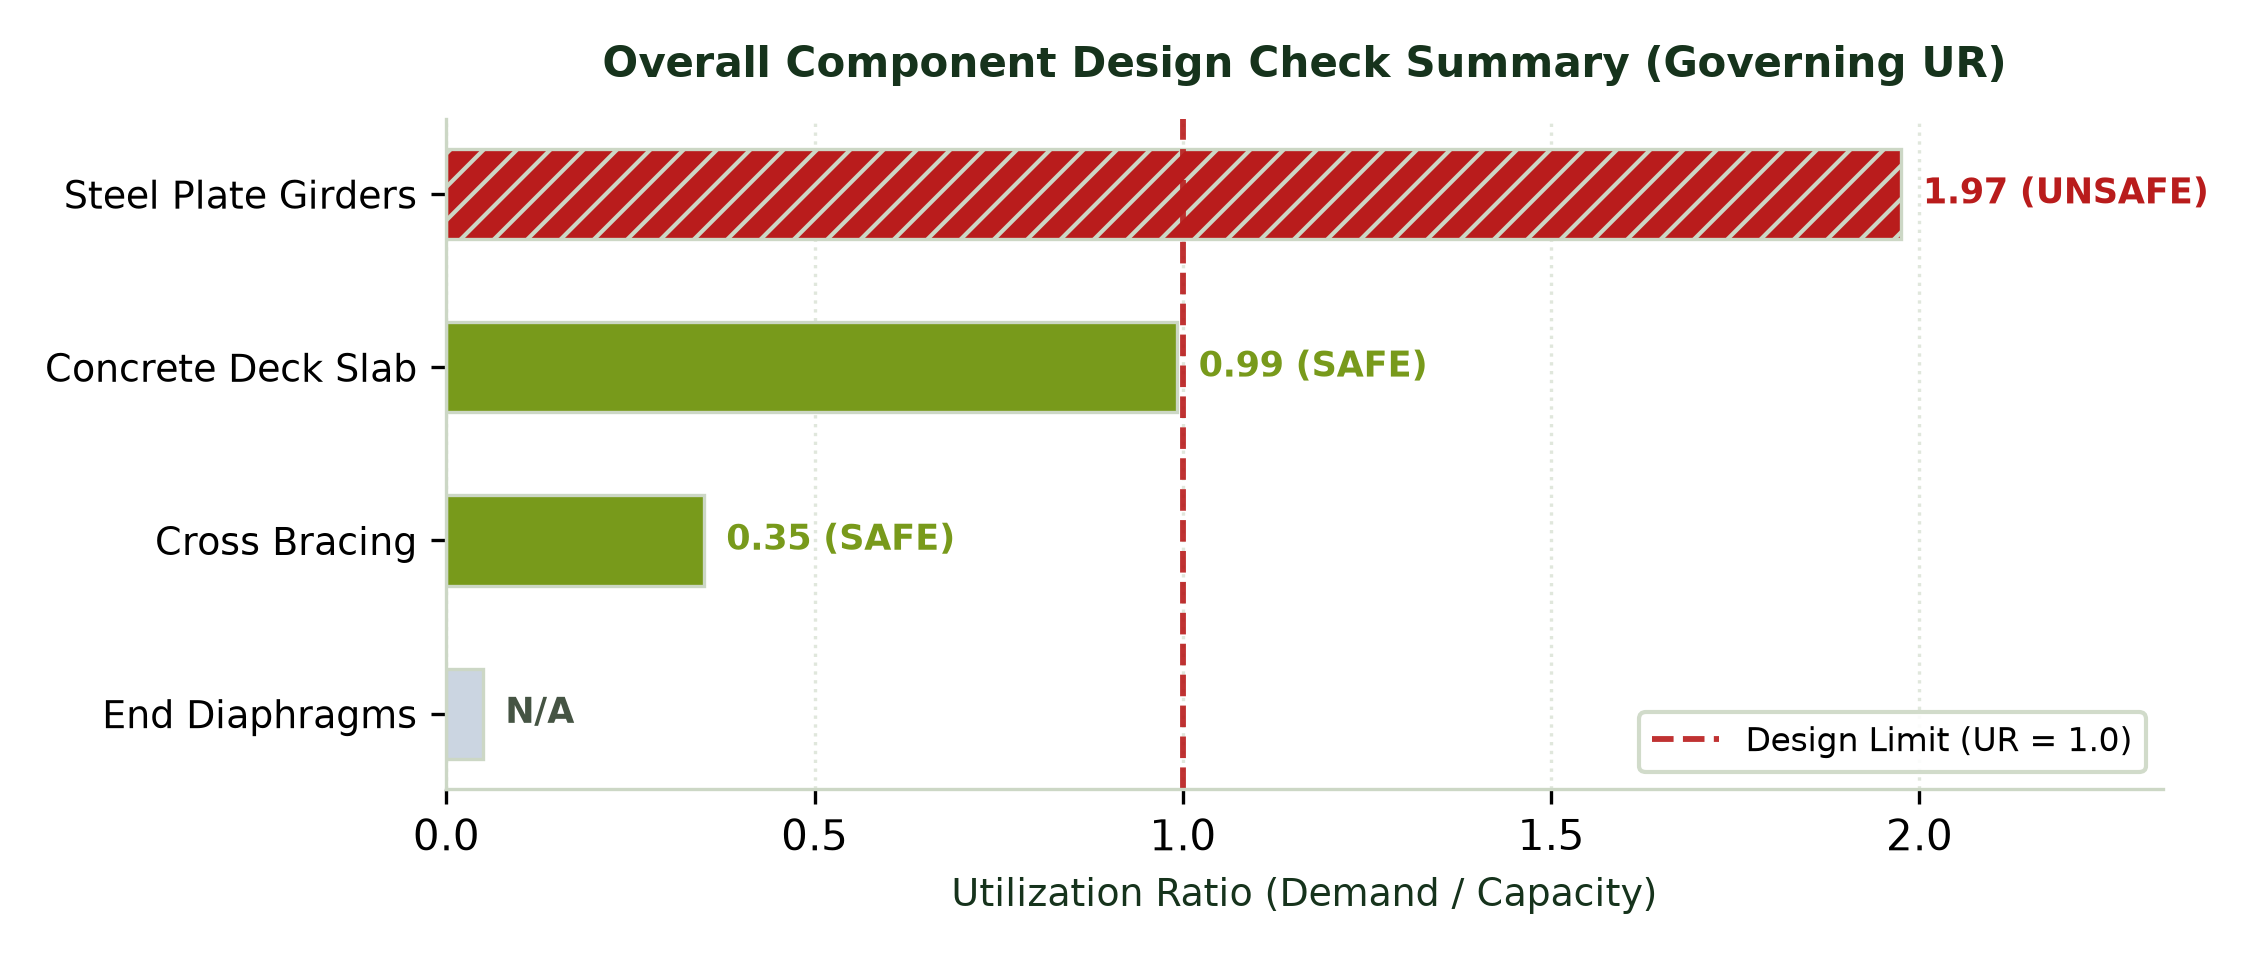
\includegraphics[width=0.95\textwidth]{assets/overall_ur_summary.png}
\caption{Overall Component Utilization Ratio (UR) Summary}
\label{fig:overall-ur-summary}
\end{figure}

\vspace{1em}
\needspace{8\baselineskip}
\setlength{\tabcolsep}{4.0pt}
\setlength\LTleft{0pt}
\setlength\LTright\fill
\begin{longtable}{|C{3.4cm}|L{4.5cm}|C{2.3cm}|C{2.3cm}|>{\centering\arraybackslash}p{1.6cm}|}
\caption{\textbf{Overall Design Check Summary - All Members}}\label{tab:overall-design-summary} \\
\hline
\rowcolor{OsdagHeaderBg}
\textbf{Member / Check} & \textbf{Governing Load Combo} & \textbf{Demand} & \textbf{Capacity} & \textbf{UR} \\[6pt]
\hline
\endfirsthead
\multicolumn{5}{c}{\small\textit{Overall Design Check Summary - All Members (continued from previous page)}} \\[4pt]
\hline
\rowcolor{OsdagHeaderBg}
\textbf{Member / Check} & \textbf{Governing Load Combo} & \textbf{Demand} & \textbf{Capacity} & \textbf{UR} \\[6pt]
\hline
\endhead
\hline
\multicolumn{5}{r}{\small\textit{Continued on next page}} \\
\endfoot
\hline
\endlastfoot
Girder - Moment & ACCIDENTAL\_\allowbreak{}1:\allowbreak{} 1.0DL + 1.0DW + 0.75LL & 1526.50 kNm & 6495.57 kNm & 0.23 \\[6pt]
\hline
Girder - Shear & ACCIDENTAL\_\allowbreak{}1:\allowbreak{} 1.0DL + 1.0DW + 0.75LL & 304.97 kN & 460.01 kN & 0.66 \\[6pt]
\hline
Girder - LTB (constr.) & SW & 85.11 kNm & 479.69 kNm & 0.18 \\[6pt]
\hline
Girder - Deflection & 1.0 DL + 1.0 LL & 22.15 mm & 40.00 mm & 0.55 \\[6pt]
\hline
Girder - Stress & SLS\_\allowbreak{}RARE\_\allowbreak{}1:\allowbreak{} 1.0DL + 1.2DW + 1.0LL + 0.6WL & 102.79 MPa & 315.00 MPa & 0.33 \\[6pt]
\hline
Girder - Fatigue & SLS\_\allowbreak{}FREQUENT\_\allowbreak{}1:\allowbreak{} 1.0DL + 1.2DW + 0.75LL + 0.5WL & 182.63 MPa & 92.49 MPa & \textbf{\color{OsdagFail}{1.97}} \\[6pt]
\hline
Transverse Shear (slab) & - & - & - & - \\[6pt]
\hline
Crack Width (slab) & SLS\_\allowbreak{}FREQUENT\_\allowbreak{}1:\allowbreak{} 1.0DL + 1.2DW + 0.75LL + 0.5WL & 0.212 mm & 0.300 mm & 0.71 \\[6pt]
\hline
Deck - Flexure (sagging) & Basic ULS: 1.35DL + 1.5LL & 45.94 kN-m/m & 52.23 kN-m/m & 0.88 \\[6pt]
\hline
Deck - Flexure (hogging) & Basic ULS: 1.35DL + 1.5LL & 34.46 kN-m/m & 40.16 kN-m/m & 0.86 \\[6pt]
\hline
Deck - Cantilever Overhang & Basic ULS: 1.35DL + 1.5LL & 101.57 kN-m/m & 108.27 kN-m/m & 0.94 \\[6pt]
\hline
Deck - Punching Shear & Basic ULS: 1.35DL + 1.5LL & 0.19 MPa & 0.55 MPa & 0.34 \\[6pt]
\hline
Deck - One-Way Shear & Basic ULS: 1.35DL + 1.5LL & 89.24 kN/m & 107.58 kN/m & 0.83 \\[6pt]
\hline
Cross Bracing - Compression & 1.5 EQ (b) & 6.44 kN & 18.400 kN & 0.35 \\[6pt]
\hline
Cross Bracing - Tension & 1.5 EQ (b) & 4.05 kN & 45.000 kN & 0.09 \\[6pt]
\hline
Cross Bracing - Slenderness & - & 126.2 & 250 & 0.50 \\[6pt]
\hline
End Diaphragm - Compression & - & - & - & - \\[6pt]
\hline
End Diaphragm - Tension & - & - & - & - \\[6pt]
\hline
\end{longtable}
\noindent\textit{Note: UR = Demand / Capacity. All values $\leq 1.0$ indicate passing checks. The governing check for each component is highlighted in the individual design check sections above.}



\chapter{Drawings and Visualizations}
\label{ch:drawings}

This section presents CAD-generated views of the designed bridge and its components. All views are generated automatically by OsdagBridge using pythonOCC.

\section{Bridge Configuration and Layout}
\label{sec:bridge-layout}

\begin{figure}[H]
\centering
\vspace{4pt}
\includegraphics[width=0.85\textwidth]{/tmp/tmpo186htwv/images/final_geometry.png}
\caption{Overall 3D Bridge Superstructure}
\label{fig:bridge-3d}
\end{figure}


\begin{figure}[H]
\centering
\vspace{4pt}
\includegraphics[width=0.85\textwidth]{/tmp/tmpo186htwv/images/cross_section.png}
\caption{Typical Cross Section}
\label{fig:cross-section}
\end{figure}


\begin{figure}[H]
\centering
\vspace{4pt}
\includegraphics[width=0.85\textwidth]{/tmp/tmpo186htwv/images/girder_top.png}
\caption{Top View}
\label{fig:top-view}
\end{figure}


\section{Plate Girder - Detailed Views}
\label{sec:girder-views}

\begin{figure}[H]
\centering
\vspace{4pt}
\includegraphics[width=0.85\textwidth]{/tmp/tmpo186htwv/images/girder_3d.png}
\caption{3D View of Plate Girders}
\label{fig:girder-3d}
\end{figure}


\begin{figure}[H]
\centering
\vspace{4pt}
\includegraphics[width=0.85\textwidth]{/tmp/tmpo186htwv/images/section_preview.png}
\caption{Cross Section of Plate Girder}
\label{fig:girder-xsec}
\end{figure}


\begin{figure}[H]
\centering
\vspace{4pt}
\includegraphics[width=0.85\textwidth]{/tmp/tmpo186htwv/images/stiffener_preview.png}
\caption{Side View of Girder}
\label{fig:girder-side}
\end{figure}


\section{Cross Bracing Detail}
\label{sec:bracing-detail}

\begin{figure}[H]
\centering
\vspace{4pt}
\includegraphics[width=0.85\textwidth]{/tmp/tmpo186htwv/images/cb_diagram.png}
\caption{Cross Bracing Layout}
\label{fig:cb-layout}
\end{figure}


\noindent
\begin{minipage}[t]{0.31\textwidth}
\centering
\includegraphics[width=\linewidth]{/tmp/tmpo186htwv/images/cb_bracing.png}
\captionof{figure}{Cross Bracing - Bracing Section}
\label{fig:cb-bracing-sec}
\end{minipage}
\hfill
\begin{minipage}[t]{0.31\textwidth}
\centering
\includegraphics[width=\linewidth]{/tmp/tmpo186htwv/images/cb_top_chord.png}
\captionof{figure}{Cross Bracing - Top Chord Section}
\label{fig:cb-top-chord}
\end{minipage}
\hfill
\begin{minipage}[t]{0.31\textwidth}
\centering
\includegraphics[width=\linewidth]{/tmp/tmpo186htwv/images/cb_bottom_chord.png}
\captionof{figure}{Cross Bracing - Bottom Chord Section}
\label{fig:cb-bottom-chord}
\end{minipage}
            

\section{End Diaphragm Detail}
\label{sec:diaphragm-detail}

\begin{figure}[H]
\centering
\vspace{4pt}
\includegraphics[width=0.85\textwidth]{/tmp/tmpo186htwv/images/ed_diagram.png}
\caption{End Diaphragm Layout}
\label{fig:ed-layout}
\end{figure}


\noindent
\begin{minipage}[t]{0.31\textwidth}
\centering
\includegraphics[width=\linewidth]{/tmp/tmpo186htwv/images/ed_bracing.png}
\captionof{figure}{End Diaphragm - Bracing Section}
\label{fig:ed-bracing-sec}
\end{minipage}
\hfill
\begin{minipage}[t]{0.31\textwidth}
\centering
\includegraphics[width=\linewidth]{/tmp/tmpo186htwv/images/ed_top_chord.png}
\captionof{figure}{End Diaphragm - Top Chord Section}
\label{fig:ed-top-chord}
\end{minipage}
\hfill
\begin{minipage}[t]{0.31\textwidth}
\centering
\includegraphics[width=\linewidth]{/tmp/tmpo186htwv/images/ed_bottom_chord.png}
\captionof{figure}{End Diaphragm - Bottom Chord Section}
\label{fig:ed-bottom-chord}
\end{minipage}



\chapter{Material Take-off \& Quantity Summary}
\label{ch:material-takeoff}

This chapter details the quantitative bill of materials (BoQ) for structural steel, concrete, reinforcement, and accessories, accompanied by visual component-level distribution charts.

\section{Material Breakdown Charts}
\label{sec:material-charts}

\begin{figure}[H]
\centering
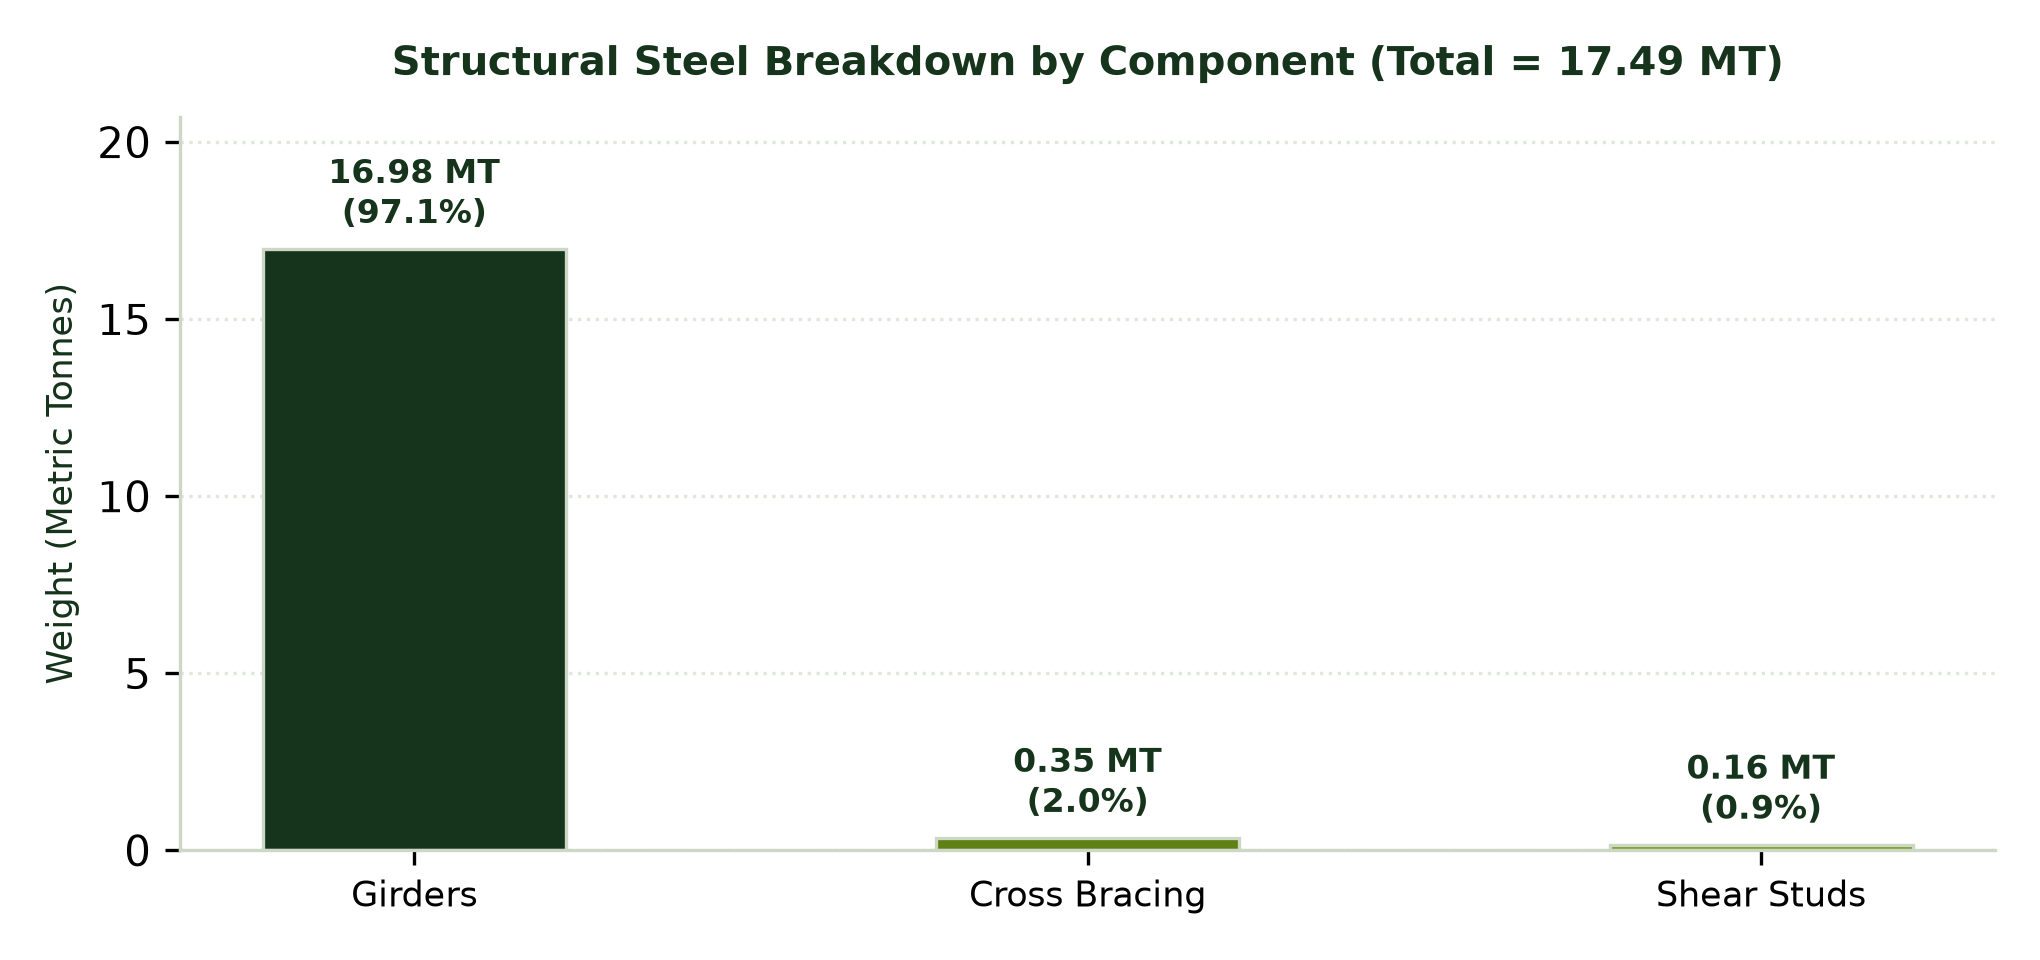
\includegraphics[width=0.92\textwidth]{assets/material_steel_breakdown.png}
\caption{Structural Steel Tonnage Breakdown by Superstructure Component}
\label{fig:material-steel-breakdown}
\end{figure}

\vspace{0.5em}

\begin{figure}[H]
\centering
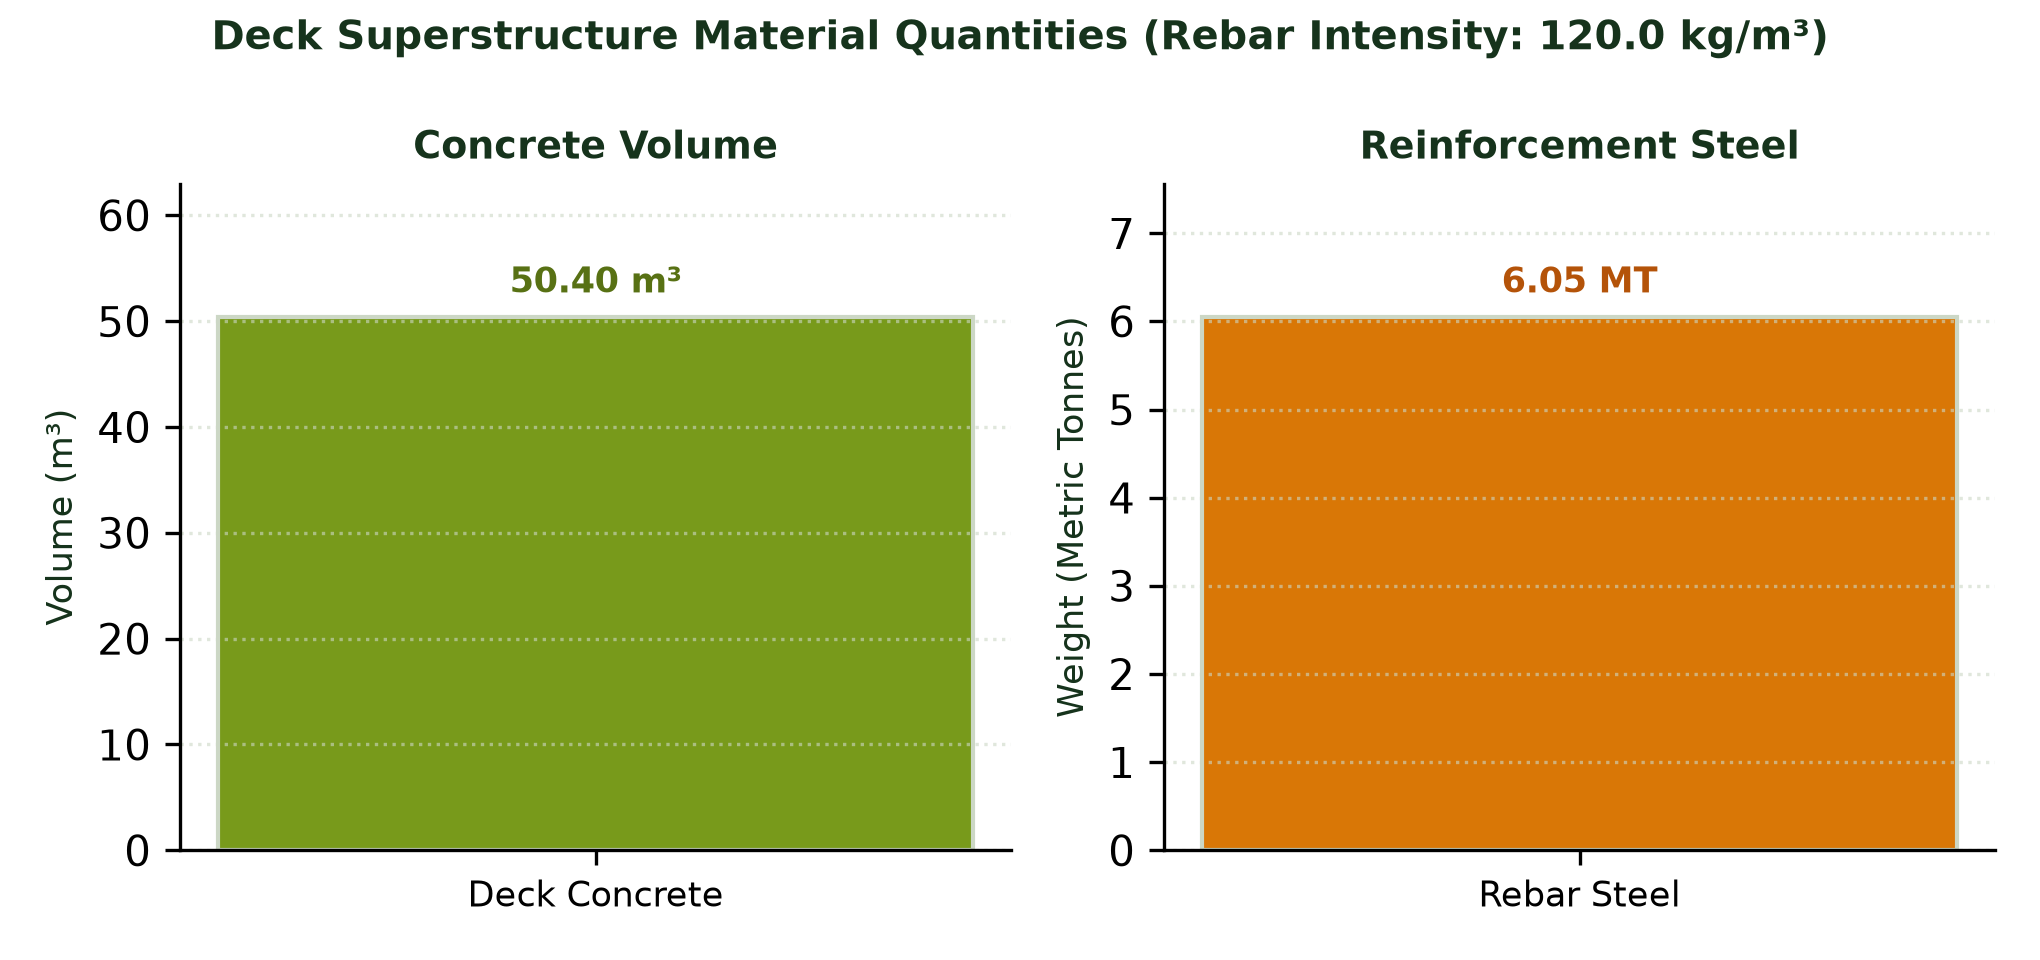
\includegraphics[width=0.92\textwidth]{assets/material_concrete_rebar.png}
\caption{Deck Superstructure Concrete Volume and Reinforcement Steel Take-off}
\label{fig:material-concrete-rebar}
\end{figure}

\clearpage
\section{Bill of Materials}
\label{sec:bill-of-materials}

\begingroup
\setlength{\tabcolsep}{3.5pt}
\setlength\LTleft{0pt}
\setlength\LTright\fill
\begin{longtable}{|C{0.9cm}|L{3.0cm}|C{4.2cm}|C{1.1cm}|C{1.6cm}|C{1.6cm}|C{1.6cm}|}
\caption{\textbf{Bill of Materials (Steel, Concrete, and Reinforcement Quantities)}}\label{tab:bill-of-materials} \\
\hline
\rowcolor{OsdagHeaderBg}
\makecell{\textbf{S.N.}} & \makecell{\textbf{Item Description}} & \makecell{\textbf{Volume}} & \makecell{\textbf{Qty}} & \makecell{\textbf{Total}\\\textbf{Vol (m$^3$)}} & \makecell{\textbf{Unit}\\\textbf{Wt (MT)}} & \makecell{\textbf{Total}\\\textbf{Wt (MT)}} \\[6pt]
\hline
\endfirsthead
\multicolumn{7}{c}{\small\textit{Bill of Materials (continued from previous page)}} \\[4pt]
\hline
\rowcolor{OsdagHeaderBg}
\makecell{\textbf{S.N.}} & \makecell{\textbf{Item Description}} & \makecell{\textbf{Volume}} & \makecell{\textbf{Qty}} & \makecell{\textbf{Total}\\\textbf{Vol (m$^3$)}} & \makecell{\textbf{Unit}\\\textbf{Wt (MT)}} & \makecell{\textbf{Total}\\\textbf{Wt (MT)}} \\[6pt]
\hline
\endhead
\hline
\multicolumn{7}{r}{\small\textit{Continued on next page}} \\
\endfoot
\hline
\endlastfoot
1 & Structural Steel (IS 2062) for Girders & \makecell[c]{\footnotesize $0.02253\text{ m}^2 \times 24.00\text{ m}$ \\ \footnotesize $= 0.54082\text{ m}^3$} & 4 & 2.16 & 4.25 & 16.98 \\
\hline
\rowcolor{OsdagZebra}
2(a) & Cross Bracing - Top Chord & \makecell[c]{\footnotesize $0.00024\text{ m}^2 \times 2.10\text{ m}$ \\ \footnotesize $= 0.00050\text{ m}^3$} & 21 & 0.01 & 0.0039 & 0.08 \\
\hline
2(b) & Cross Bracing - Bottom Chord & \makecell[c]{\footnotesize $0.00024\text{ m}^2 \times 2.10\text{ m}$ \\ \footnotesize $= 0.00050\text{ m}^3$} & 21 & 0.01 & 0.0039 & 0.08 \\
\hline
\rowcolor{OsdagZebra}
2(c) & Cross Bracing - Diagonal Chord & \makecell[c]{\footnotesize $0.00024\text{ m}^2 \times 2.39\text{ m}$ \\ \footnotesize $= 0.00057\text{ m}^3$} & 42 & 0.02 & 0.0044 & 0.19 \\
\hline
3 & Concrete (M40) for Deck Slab & \makecell[c]{\footnotesize $8.40\text{ m} \times 0.25\text{ m} \times 24.00\text{ m}$ \\ \footnotesize $= 50.40\text{ m}^3$} & 1 & 50.40 & 126.00 & 126.00 \\
\hline
\rowcolor{OsdagZebra}
4 & Reinforcement Steel (Fe 500) & \makecell[c]{\footnotesize $0.032102\text{ m}^2 \times 24.00\text{ m}$ \\ \footnotesize $= 0.77045\text{ m}^3$} & 1 & 0.77 & 6.05 & 6.05 \\
\hline
5 & Shear Stud Connectors & \makecell[c]{\footnotesize $0.000314\text{ m}^2 \times 0.100\text{ m}$ \\ \footnotesize $= 0.000031\text{ m}^3$} & 640 & 0.02 & 0.000247 & 0.158 \\
\hline
\rowcolor{OsdagZebra}
6 & Crash Barrier & \makecell[c]{\footnotesize $0.00000\text{ m}^2 \times 24.00\text{ m}$ \\ \footnotesize $= 0.00001\text{ m}^3$} & 2 & 0.00 & 0.00 & 0.00 \\
\hline
\end{longtable}
\endgroup


\chapter{Standards \& Assumptions}
\label{ch:Design Standards}

This section provides references to standards used to calibrate the OsdagBridge
design modules, and notes the limitations of the current software version.

\section{Design Standards}
\label{sec:design_standards}

The following Indian Road Congress (IRC) codes and Indian Standards (IS) 
form the basis of all design calculations in this software.

\vspace{0.5cm}

\begingroup
\setlength{\tabcolsep}{4.5pt}
\begin{table}[H]
\caption{\textbf{Indian Roads Congress (IRC) Design Codes}}
\begin{tabular}{|C{2.6cm}|C{1.8cm}|p{11.8cm}|}
\hline
\rowcolor{OsdagHeaderBg}
\textbf{Code} & \textbf{Year} & \textbf{Title / Scope} \\ 
\hline
IRC 5 & 2015 & General Features of Design - carriageway widths, kerb, footpath dimensions \\ 
\hline
\rowcolor{OsdagZebra}
IRC 6 & 2017 & Loads and Load Combinations - dead load, live load, impact, wind, temperature, etc. \\ 
\hline
IRC 22 & 2015 & Composite Construction (LS) - Composite section properties, ULS/SLS design, shear connectors \\ 
\hline
\rowcolor{OsdagZebra}
IRC 24 & 2010 & Steel Road Bridges (LS) - Stiffener design, skew angle limits, diaphragm requirements \\ 
\hline
IRC 112 & 2020 & Concrete Road Bridges - Deck slab flexure, shear, crack width, reinforcement \\ 
\hline
\rowcolor{OsdagZebra}
IRC SP 114 & 2018 & Seismic Design of Road Bridges \\ 
\hline
\end{tabular}
\end{table}
\endgroup

\begingroup
\setlength{\tabcolsep}{4.5pt}
\begin{table}[H]
\caption{\textbf{Bureau of Indian Standards (IS) Design Codes}}
\begin{tabular}{|C{2.6cm}|C{1.8cm}|p{11.8cm}|}
\hline
\rowcolor{OsdagHeaderBg}
\textbf{Code} & \textbf{Year} & \textbf{Scope} \\
\hline
IS 800 & 2007 & Steel construction - tension, compression, bending, shear, LTB, stiffeners, combined checks \\
\hline
\rowcolor{OsdagZebra}
IS 456 & 2000 & Concrete - simplified stress-block for deck moment capacity \\
\hline
IS 1786 & 2008 & Reinforcement steel properties \\
\hline
\rowcolor{OsdagZebra}
IS 1893 (Part 3) & 2014 & Earthquake resistant design \\
\hline
IS 2062 & 2011 & Structural steel - yield and ultimate strength by grade \\
\hline
\end{tabular}
\end{table}
\endgroup

\clearpage
\section{Analysis and Design Assumptions of This Version}
\label{sec:assumptions}

\textbf{Structural Analysis}

\begin{itemize}
    \item All girders are modelled as simply supported; continuous spans are not currently supported.
    \item A 3D grillage model (OSPGrillage) is used for load distribution. Grillage members carry composite section properties after the construction stage.
    \item The transverse member forces are computed using an approximate 2D frame analogy. For irregular or skewed geometries, a 3D FEM is recommended.
    \item Fixed bearing stiffness is modelled as $k = 1{,}000{,}000 \,\text{kN/m}$ (virtually rigid); free/expansion bearing as $k = 100 \, \text{kN/m}$.
    \item Construction stage sequence analysis is approximate. Detailed staged analysis should be performed for long-term deflection checks.
\end{itemize}

\textbf{Composite Action}

\begin{itemize}
    \item Full shear connection is assumed at ULS with headed stud connectors designed per IRC 22:2015 Cl.606.
    \item Short-term composite section properties (modular ratio $n = E_s/E_{cm}$) are used for ULS checks.
    \item Long-term composite section properties (with creep-adjusted modular ratio) are used for SLS deflection and crack-width checks.
    \item Pre-composite stage: the steel girder alone resists all construction loads prior to concrete gaining strength.
\end{itemize}


\textbf{Material Properties (IRC 22:2015 Annex III)}

\begin{itemize}
\item Steel: $E_s = 200{,}000 \, \text{MPa}, \ G_s = 80{,}000 \, \text{MPa}, \ \nu = 0.30, \ \alpha = 11.7 \times 10^{-6}/^\circ\mathrm{C}$ (grade-independent).
\item Minimum structural concrete grade: M25.
\item Default reinforcement grade: Fe500.
\end{itemize}

\textbf{Partial Safety Factors (IRC 22:2015 Cl.601.4)}

\begin{itemize}
\item $\gamma_{m0}$ (steel yield, ULS) = 1.10
\item $\gamma_{m1}$ (steel ultimate, ULS) = 1.25
\item Reinforcement (ULS) = 1.15
\item Welds: shop: 1.25; field: 1.50
\item Fatigue ($\gamma_{mft}$) = 1.35
\end{itemize}

\textbf{Loading}

\begin{itemize}
\item Dead load densities per IRC 6:2017 Cl.203: structural steel $78.5 \ \text{kN/m}^3$, concrete $25.0 \ \text{kN/m}^3$, bituminous wearing course $24.0 \ \text{kN/m}^3$.
\item Multi-lane live load reduction factors per IRC 6:2017 Cl.204.4 Table 6A: 1st lane = 1.0, 2nd lane = 0.8, 3rd lane onwards = 0.4.
\item Impact factor (dynamic load allowance) computed from span per IRC 6:2017 Cl.208.2/208.3.
\item Wind load applied as transverse, longitudinal, and vertical components per IRC 6:2017 Cl. 209.3.3 to 209.3.5.
\end{itemize}

\textbf{Serviceability Limits}

\begin{itemize}
\item Deflection limits (IRC 22:2015 Cl.604.3.2): live load + impact $\leq L/800$; total $\leq L/600$.
\item SLS stress limits: concrete $\sigma_c \leq 0.48 f_{ck}$; rebar $\sigma_s \leq 0.80 f_{yk}$; steel $f_e \leq 0.9 f_y$.
\item Permissible crack width: $w_k \leq 0.3 \ \text{mm}$ (bridge deck, exposure class XS2/XD2 per IRC 112:2020 Cl.12.3.2).
\end{itemize}

\textbf{Fatigue}

\begin{itemize}
\item Reference fatigue life: $N_{sc} = 2 \times 10^6$ cycles (IRC 22:2015 Cl.605).
\item Constant stress range is assumed. A thickness correction factor $\mu_r$ is applied for plate thickness $> 25 \ \text{mm}$.
\end{itemize}

\textbf{Stiffener Design}

\begin{itemize}
\item Intermediate transverse stiffener and bearing stiffener design follows IS 800:2007 Cl.8.7.2/8.7.3 and IRC 24:2010 Cl.509.7.2/509.7.3.
\end{itemize}


\section{Known Limitations of This Version}
\label{sec:limitations}

\begin{itemize}
\item Substructure (piers, pile caps, foundations) and bearing design are not included.
\item Splice connection design is not implemented.
\item Skew angle $>$ 15 degrees requires independent manual analysis (IRC 24 Cl. 504.8).
\item Construction stage sequence analysis is approximate; detailed staged analysis
  should be performed for long-term deflection checks.
\item The grillage analysis assumes simply supported boundary conditions;
  continuous spans are not currently supported.
\end{itemize}


\chapter*{References}
\addcontentsline{toc}{chapter}{References}


\begin{enumerate}

\item IRC 5 (2015): \textit{Standard Specifications and Code of Practice for Road Bridges, Section I: General Features of Design.}

\item IRC 6 (2017): \textit{Standard Specifications and Code of Practice for Road Bridges, Section II: Loads and Load Combinations.}

\item IRC 22 (2015): \textit{Standard Specifications and Code of Practice for Road Bridges, Section VI: Composite Construction (Limit State Design).}

\item IRC 24 (2010): \textit{Standard Specifications and Code of Practice for Road Bridges, Section V: Steel Road Bridges (Limit State Method).}

\item IRC 112 (2020): \textit{Code of Practice for Concrete Road Bridges.}

\item IRC SP 114 (2018): \textit{Guidelines for Seismic Design of Road Bridges.}

\item IS 800 (2007): \textit{Indian Standard: General Construction in Steel - Code of Practice.}

\item IS 2062 (2011): \textit{Hot Rolled Medium and High Tensile Structural Steel - Specification.}

\item Subramanian, N. (2008). \textit{Design of Steel Structures.} Oxford University Press.

\item Steel-INSDAG Teaching Resource Materials. \url{https://www.steel-insdag.org}

\end{enumerate}

\end{document}